%
% File acl2019.tex
%
%% Based on the style files for ACL 2018, NAACL 2018/19, which were
%% Based on the style files for ACL-2015, with some improvements
%%  taken from the NAACL-2016 style
%% Based on the style files for ACL-2014, which were, in turn,
%% based on ACL-2013, ACL-2012, ACL-2011, ACL-2010, ACL-IJCNLP-2009,
%% EACL-2009, IJCNLP-2008...
%% Based on the style files for EACL 2006 by 
%%e.agirre@ehu.es or Sergi.Balari@uab.es
%% and that of ACL 08 by Joakim Nivre and Noah Smith

\documentclass[11pt,a4paper]{article}
\usepackage[hyperref]{acl2019}
\usepackage{times}
\usepackage{latexsym}
\usepackage{graphicx}
\usepackage{amsmath}
\usepackage[utf8]{inputenc}
\usepackage{xspace}
\usepackage{paralist}
\usepackage{booktabs}
%\usepackage{pdfpages}

\usepackage{tikz}
\usepackage{tikz-qtree}

\usepackage{url}
\usepackage[normalem]{ulem}

\aclfinalcopy % Uncomment this line for the final submission
\def\aclpaperid{BlackboxNLP 31}  %  Enter the acl Paper ID here

%\setlength\titlebox{5cm}
% You can expand the titlebox if you need extra space
% to show all the authors. Please do not make the titlebox
% smaller than 5cm (the original size); we will check this
% in the camera-ready version and ask you to change it back.

\newcommand\BibTeX{B\textsc{ib}\TeX}
\newcommand\eg{e.g.\ }
\newcommand\ie{i.e.\ }
\newcommand\footurl[1]{\footnote{\url{#1}}}

% how to call the input and output positions
% input, i.e. attended to:
\newcommand{\word}{\emph{input state}\xspace}
\newcommand{\words}{\emph{input states}\xspace}
% output, i.e. they attend to input:
\newcommand{\state}{\emph{output state}\xspace}
\newcommand{\states}{\emph{output states}\xspace}

\def\RR#1{{\color{blue}RR: \it #1}}
\def\DM#1{{\color{red}DM: \it #1}}
\def\JL#1{{\color{magenta}JL: \it #1}}
\def\JLrepl#1#2{{\color{magenta}JL: \sout{#1} \it #2}}
\def\DEL#1{{\color{green}SMAZAT: \it #1}}
\def\REC#1{{\color{cyan}REC: \it #1}}
\def\JL#1{}
\def\JLrepl#1#2{}
\def\RR#1{}
\def\DM#1{}
\def\DEL#1{}

\title{From Balustrades to Pierre Vinken:\\Looking for Syntax in Transformer Self-Attentions}

\author{David Mare\v{c}ek \and Rudolf Rosa\\
  Charles University, Faculty of Mathematics and Physics \\
  Institute of Formal and Applied Linguistics \\
  Malostransk\' e n\' am\v est\' i 25, 118 00 Prague, Czech Republic \\
  \texttt{\{marecek, rosa\}@ufal.mff.cuni.cz}}

\date{}

\begin{document}
\maketitle
\begin{abstract}
%We pose ourselves the question whether syntax-like structures emerge in Deep Neural Networks trained to process language, as has been suggested by previous authors.
%In this study, we
We inspect the multi-head self-attention in Transformer NMT encoders for three source languages, looking for patterns that could have a syntactic interpretation. In many of the attention heads, we frequently find sequences of consecutive states attending to the same position, which resemble syntactic phrases.
We propose a transparent deterministic method of quantifying the amount of syntactic information present in the self-attentions,
based on automatically building and evaluating phrase-structure trees from the phrase-like sequences.
%To keep our primary method linguistically uninformed, we use all attention heads. However, we also introduce and analyze a contrastive approach, in which we attempt to automatically identify and use only the ``syntactic'' attention heads.
We compare the resulting trees to existing constituency treebanks, both manually and by computing precision and recall.
\end{abstract}

\section{Introduction}

%\RR{subword or sub-word?} \JL{Rico to píše bez pomlčky}

%\RR{TODO kdekoliv mam v textu nějaký čísla (něco je třetina něčeho atd.) tak jsou spíš odhadnutý a neni jim co věřit, měly by se zkontrolovat}

The classical approach to Natural Language Processing used to be complex
pipelines, e.g.~\cite{tectomt:2010, manning:2014, apertium:2011},
%\JL{to chce další příklady, třeba Stanfordí correference resolver 2014}
consisting of multiple steps of linguistically motivated analyses,
such as part-of-speech tagging or syntactic parsing, using explicit
intermediate representations (\eg dependency trees) to abstract over the underlying texts.

In recent years, this has changed with the introduction of deep neural
end-to-end models, which take raw text as input and produce the desired
output directly. Any intermediate representations of the text
may
%latently
emerge during the training of the neural
network, and are hidden to us.
% nějak vysvětlit že tam vznikaj bez toho abychom my je tam vynucovali nebo dokonce řikali jak maj vypadat; ale možná už to z toho je takhle zřejmé

%There is a number of questions many have been asking.
%What are these latent
%representations? What do they capture? Can we understand them? In what ways
%are they similar to the classical linguistic representations that we know? Do
%they capture interesting language phenomena?
%In our research, we are asking ourselves the same questions.
%\JL{Tohle si schovej do úvodní kapitoly knihy.}

We focus on the encoder part of the Transformer architecture \cite{vaswani2017attention}, applied to neural machine translation (NMT),
%one linguistic phenomenon.
%In introducing the Transformer architecture,
as
visualizations presented by the authors suggest that its attention heads capture various phenomena such as syntax, semantic roles or anaphora links.
%We focus on syntactic properties of the attention head.

In this work, we analyze the syntactic properties of the self-attention heads both qualitatively and quantitatively. For the quantitative evaluation, we devise a new technique that quantifies
the amount of syntactic information by explicitly building constituency trees from the attentions and comparing them
with the standard syntactic trees.
%human annotation.
%\DM{a jeste o tom vyberu syntaktickych hlav}

%\citet{vaswani2017attention} have
%shown visualizations of two self-attention heads indicating that they seem to capture something similar to syntax. We are not aware of any follow-up work that
%would inspect the self-attention in more detail and from the syntactic point of view. We investigate this in a more principled way, examining attention matrices for all layers and heads of standard self-attentive Transformer encoders, trained for the task of machine translation between various pairs of European languages.


%The main contributions of this paper are: \JL{Má to začínat tím To?}
%
%\begin{itemize}
%
%    \item To make thorough analysis of the encoder self-attentions.
%
%    \item To introduce a method how to build constituency trees solely based on the self-attention 
%   information and compare them to manually annotated treebanks.
%
%\end{itemize}

%\JL{To není v souladu s abstraktem, kde tvrdíte, že kvantifikujete, kolik syntaxe je v těch attentionech. Jatože to není najednou contribution? Předchozí odstavce bych nahradil mým krátkým odtsavečekm.}

Section~\ref{sec:visualization} briefly describes the Transformer encoder architecture and the way we
visualize the self-attention matrices using heatmaps.
In Section~\ref{sec:analysis}, we present our findings from an extensive manual inspection of the
heatmaps, identifying several common patterns, including the baluster-like
structures which seem to resemble syntactic phrases.
%However, the eye can be deceitful, \JL{a cesty páně jsou nevyzpytatelné} seeing what it wants to see.
%\JL{Smazat.}For us, our manual analysis is rather an exploratory pre-stage, guiding our
%further and more reliable examination.\JL{až sem.}
To avoid
%fooling ourselves
confirmation bias, we proceed by devising a
%transparent
%linguistically uninformed deterministic non-trained syntactic parsing algorithm 
linguistically uninformed tree extraction algorithm
(Section~\ref{sec:parsing}), which
builds a constituency tree
%using the CKY algorithm~\cite{ney:1991}
based solely on the assumption that the balusters
correspond to syntactic phrases.
We analyze the resulting parse trees and compare them with standard
%Penn Treebank style
syntactic
trees, both manually and via automatic evaluation. %(Section~\ref{sec:results}).
%\DM{TODO: je treba doplnit tu manual evaluation}
%
In Section~\ref{sec:head-selection}, we follow the hypothesis that only some of the attention heads
are ``syntactic'', and try to identify them.
%. We perform selection of heads maximizing the scores of the resulting trees.

\DEL{ both supervisedly and heuristically
in Section~\ref{sec:head-selection},
but we do note that we may now again be performing wishful observations, as we
are seeking for the syntax quite eagerly. \JL{týhle větě nerozumim}}
%\DM{Tohle asi jeste vubec nemame, takze to dame asi pryc.}
%\RR{Myslel jsem tim že naše observations nemusej bejt až tolik observations, když natvrdo hledáme takovou kombinaci hlav aby to dobře parsovalo. Teď jdu o tom napsat tu sekci.}

%\JL{Celou následující sekci si buď schovej do knihy nebo smaž úplně. Cífka sice mulví o fixed-sozed reprezentatcích, ale delá nad nimi attention (který btw. není od sutskevera). Navíc vztah attentionu a alignmentu není jednoduhý viz (Koehn: Sxi challenges for NMT). Navíc, kde se vzal attention mi nepřijde pro váš článek relevantní.}
%\RR{
%\subsection{From word-alignment to self-attention - tohle se asi bude muset zkratit a je otazka, kam to dat}
%
%TODO tohle možná patří spíš do intra?
%
%In classical phrase-based statistical machine translation (SMT) CITE KOEHN KNIHA, word alignment was central to the approach. Based on the idea that particular words in the source language sentence correspond to particular words in the target language sentence, explicit hard alignment links were devised and parallel phrases extracted from the training data. At inference, the translation model suggested several potential translations for each source phrase, independent on any context. To produce a fluent translation, a source-uninformed language model was used, ensuring that each target phrase fits the context of the surrounding target phrases but disregarding the source completely.
%
%In classical neural machine translation (NMT), the \emph{decoder} which generates the translation is, in principle, a source-informed language model.
%While a fixed-size source-sentence representation can be used to inform the decoder, the results are rather poor CITE CIFKA:
%even though knowing the whole source sentence is useful for the decoder, the translation is still in its nature mostly a word-based or phrase-based task, as most output words directly correspond to certain source words.
%Therefore, CITE SUTSKEVER devised the attention mechanism, which is a kind of neural latent soft word-alignment. The decoder can use the attention mechanism to bring in information about one or several source words when trying to produce the right target word;
%typically, but not always, the decoder would attend to source words that would be word-aligned to this target word in classical SMT.
%
%A notable difference between word alignment and attention is that word alignment operates on words, while the attention mechanism operates on hidden states of the encoder, typically a bi-directional RNN.
%It is thus technically incorrect to say that the decoder attends to source \emph{words}, as the encoder hidden states do not have to correspond to the individual words. Theoretically, information about each input word may be pushed around and shifted and swapped and scattered by the encoder over any or all of the hidden states.
%However, in practice, this does not seem to happen too much -- the information seems to get dispersed mostly locally, and most of the information about the underlying word seems to stay put.  We thus believe it to be reasonable to think about each hidden state as a representation of the underlying word in the context of the source sentence.
%
%Theoretically, the decoder can attend to any relevant words in the source sentence. For example, when producing a target verb, it would make sense to attend both to the source verb as well as to the source subject, so as to be able to inflect the target verb appropriately. In practice, this does not happen too much, partially probably due to the particular way attention is implemented, where the representations of all of the words that are attended to are combined via a weighted average, making it harder for the decoder to separate them again.
%The task of incorporating information about relevant context from the sentence is thus mostly left to the encoder. While modern RNN cells, such as LSTMs CITE or GRUs CITE, are to some extent capable of capturing information even from tokens placed further away, they still seem to mostly only include information about the immediate context.
%}

%Transformer CITE is a state-of-the-art neural network architecture for various tasks, including machine translation.
%Its architecture is inspired by the attention mechanism, devised by CITE for a machine translation decoder to be able to specifically attend to individual words in the input sentence, similarly to how classical phrase-based machine translation decoder uses word alignment. The general idea was that to produce a particular word of the translation, 

\section{Related Work}
\label{sec:related-work}
%Majority of works analyzing neural networks with respect to learning syntax focus on recurrent network (RNN) architectures.
Initial analyses of syntax captured by neural networks focused on RNNs.
\citet{shi:padhi:knight:2016} examine how much syntax is learned by RNN encoder by freezing
%encoder's
its
weights and using a decoder to predict syntactic trees.
\citet{adi:2016} examine sentence vector representations by training auxiliary classifiers to take sentence encodings and predict attributes like word order.
\citet{linzen2016assessing} assess the ability of LSTMs to learn syntax by predicting verbal numbers. 
\citet{blevins-levy-zettlemoyer:2018} measure the amount of syntax in RNNs by predicting part-of-speech tags and constituent labels.
%, and parent's and gradparent's constituent labels.
% \citet{belinkov:2018} -- ale to je RNN a neni to syntax

In the last year, related studies appeared also for the Transformer architecture.
\citet{tang:2018} show the Transformer networks perform better than RNNs on
word sense disambiguation.
%Dělal nějakou adversarial evaluation, která ukázala, že Transformír je pro syntax nejleší.
%\cite{ahmed:2017}
%Weighted Transformer Network for Machine Translation
\citet{zhang:2018} show that language models use more syntactic and morphological information than translation models.
%\DM{\citet{vaswani2017attention} show examples of two attention heads which seem to exhibit syntactic behaviour, but we are unaware of any existing deeper analysis of this phenomenon. This forms the core of our work.}


%\citet{belinkov:phd:2018}

Recently, \citet{hewitt:2019} tried to find syntactic structures in contextual word representations by training simple models on annotated parse trees, concluding that syntactic trees are embedded both in BERT \citep{bert} and ELMo \citep{elmo} models.
This is also supported by \citet{belinkov:2019}, who successfully trained probes to extract linguistic structures, including syntactic dependencies, from various trained neural networks.

Most existing works train probing models on annotated data (e.g.\ treebanks).
%With such models, there is always a threat that the model learns
However, such a model may learn
to predict the linguistic structure not because it is captured by the network, but because it can be predicted from features
preserved from the input,
%of the input that are preserved by the neural encoder,
as has been already noted e.g.\ by \citet{belinkov:survey}.
In our work, we try to avoid that risk by not using annotated data for the predictions, but rather looking for structures explicitly present in the network representations.
%We may thus underestimate the amount of linguistic information captured by the network, but we strongly believe that we are not overestimating it.

% \RR{TODO tohle zkrátit (ale nějak to sem asi dát):}

% As noted e.g.\ by \citet{belinkov:survey}, the fact that some information seems to be encoded in a network does not necessarily mean that the network uses that information. It may simply be that the information, already implicitly present in the input, is not lost by the encoding.
% We believe that the risk of such misinterpretation is higher with probing models trained with annotated data, as is the case with most existing studies, and increases with the complexity of the model.
% Therefore, we take the opposite approach, not training any model and not using annotated data except for evaluation, but simply looking for what is rather explicitly present in the representations without further custom transformations.
% We thus run the opposite risk of underestimating the amount of linguistic information captured by the network, but we are quite confident that any linguistic information that we find is really there.

%\DM{pridat Belinkova a Hewitta a Manninga}

\RR{Tady je zakomentovaný relwork z Hewitta}

% HEWITT RELATED WORK -- KOPIE Z ČLÁNKU ALE MŮŽE TO BEJT RELEVANTNÍ
% Our work extends the
% literature on linguistic probes, found at least in (Peters et al., 2018b; Belinkov et al., 2017; Blevins
% et al., 2018; Hupkes et al., 2018). Conneau et al.
% (2018) present a task similar to our parse depth
% prediction, where a sentence representation vector
% is asked to classify the maximum parse depth ever
% achieved in the sentence. Tenney et al. (2019) evaluates a complementary task to ours, training probes
% to learn the labels on structures when the gold structures themselves are given. Peters et al. (2018b)
% evaluates the extent to which constituency trees can
% be extracted from hidden states, but uses a probe
% of considerable complexity, making less concrete
% hypotheses about how the information is encoded.

In a study closely related to ours,
\citet{raganato:2018} also observe syntax-like patterns in Transformer encoder self-attentions, and try to extract syntactic trees without using annotated data (except for taking the root node from the gold annotation).
However, they construct dependency trees, while we observe phrase-like rather than dependency-like structures.
Moreover, their findings are somewhat inconclusive,
as the accuracy of the resulting trees is close to the
%right-branching
baseline,
while our results are clearly positive.
A similar approach was already suggested (but not evaluated) in \citep{marecek:blackbox2018}.

% To the best of our knowledge, the recent work of \citet{raganato:2018} is the only one so far that has delved deeper into investigating the syntactic structures that may be present in Transformer encoder self-attentions.
% They try to interpret the attention points as syntactic dependency edges, using the attention weights as edge weights, and inducing a dependency tree using the Maximum Spanning Tree algorithm of~\citet{chuliu}.
% However, there
% %does not seem to be a
% is no
% straightforward way of identifying the root of the syntactic tree based on the attentions, which the authors circumvent by using the root from the gold syntactic annotation.

% %Unlike \citet{raganato:2018},
% In our work,
% we extract constituency trees instead,
% as we observed phrase-like rather than dependency-like structures in the attentions.
% %we observe remarkably phrase-like structures in the attentions, rather than dependencies, and thus decided to extract constituency trees.
% Furthermore, we combine information from all of the attention heads, while \citet{raganato:2018} use each head separately.
% While their findings are somewhat inconclusive,
% %Their findings are somewhat inconclusive,
% %as
% the resulting trees
% being
% %are
% approximately as good as the right-branching baseline,
% our results are clearly positive.




%And finally, our results are much more positive.

%Our work differs from \citep{raganato:2018} in several ways.
%The key difference is that based on the inspection of the attentions, we decided to search for phrase structure trees rather than dependency trees, since we have observed remarkably phrase-like structures in the attention visualisations while not really observing clearly dependency-like structures.
%Also, we induce the syntactic trees based on a combination of information from all of the attention heads, while the previous authors used each head separately.
%We also focus solely on the problem of looking for syntactic structures, focusing on depth, while the previous autors focused on breadth, analyzing the attentions in several other ways, unrelated to syntax.
%\RR{TOHLE ZNÍ BLBĚ ALE JAK TO ŘÍCT? Eventually, our findings seem to be much more convincing then theirs.}

%\JL{ještě Rico Sennrich měl teď na EMNLP: Why self-attention? }

\JL{asi by se taky hodilo zmínit, že Transormerem jde dělat i parsing https://arxiv.org/pdf/1807.03819.pdf, https://arxiv.org/pdf/1706.05137.pdf
a navíc teď  vyšel BERT, kterej ukazuje, že když dobře naučíš transformíra, tak v tý reprezentaci 
najdeš cokoli}

\section{Transformer NMT Encoder}
\label{sec:visualization}

In the Transformer architecture, \citet{vaswani2017attention} came up with several important improvements over the classical attention,
%mechanism.
%Most importantly, they developed \emph{multi-headed} attention, featuring
including \emph{multi-headed} attention. It features
a set of independent attention heads, each deciding on its own to which states to attend.
%; the outputs are then concatenated instead of averaging them, making it straightforward for the subsequent network layer to discern which information comes from which of the attention heads. \JL{Tíhle tvrzením bych si nebyl tak jistý. První věc, co se s těma hlavama stane je, že se linérně smíchají nějakou váhovou maticí do dimenze modelu, pak se znormalizují, pak se přičte residual connection a pak teprve vstupjí do další opravické vrstvy. V předchozí větě smazat věci od středníku do tečky.}
This allows each of the heads to specialize to provide a different type of information or feature (similarly \eg to CNN filters).
%\RR{There may thus be a head simulating the word-alignment, several heads attending to particular positions from the local context (previous word, following word\ldots), heads providing syntactic context (phrase boundary, phrase head, dependency parent, dependency child\ldots), heads representing global features (sentence beginning, sentence end\ldots), etc.
%But all of these are just possible options we can imagine for the heads. The question, of course, is: Do the heads really specialize in these ways? What information do they capture in practice?}
%\JL{Tenhle výčet spekulací by sis taky měl schovat do knihy.}
%Moreover, in Transformer, there is the multi-head attention is not only present at the encoder-decoder boundary, but is also used as self-attention in the encoder and the decoder.
%and the decoder as well, but we do not deal with the decoder in this work).
%Instead of using a RNN or CNN to encode the source sentence,
The encoder typically uses six multi-head self-attention sub-layers.
Each state
%representing a word
%\JL{to přece neni jistý, jestli reprezntuje slovo, ještě k tomu teda subword}
on a given layer (\state) is computed from a concatenation of the result of applying a set of attention heads to the states on the previous layer (\words),
%The result of the self-attention is
passed through a feed-forward layer.
This may allow the encoder to do more advanced multi-step processing, such as aggregating the information about several subwords into one position and then attending to this position on the higher layers.

%In the following text, w
%We use the term \state for hidden states on the current layer and the term \word for the hidden states from the previous layer -- through the self-attention mechanism, the \states attend to the \words.
%(previous layer position) describing the hidden states on the previous layer, to which the \states attend.



%Transformer uses scaled dot-product attention, where a set of three vectors (\emph{Query}, \emph{Key}, \emph{Value}) is generated for each \word. The attention weight at a given position is then computed as a softmaxed dot-product of the \emph{Query} corresponding to the position of the \state and the \emph{Key} corresponding to each of the \words. The result of applying the attention is then computed by as an average of the \emph{Values} of the \words weighted by the attention weights.

Another notable feature of the Transformer encoder is the use of residual connections, which transport the source subword embeddings forward, bypassing the self-attention mechanism, and get averaged with the outputs of the self-attention.
This ensures that the \state at each position retains a significant amount of the corresponding source subword embedding, supporting the usual shortcut of assuming that the hidden states can be thought of as representations of the underlying subwords (in the context of the sentence).
%In the following text, we will thus simply say that each \state attends to \words.

%JL{Tenhle předpoklad musí zaznít před tím, že než budeš pracovat s tím, že i na dalších vrstvách ty tavy reprezentují slova.}

%\JL{v tom původní článku říkají sub-layer}

%all words that are part of one syntactic phrase onto one position, \eg the first token of the phrase, in lower layers, and then attending to this position in the higher layers, thus obtaining information not only about the first token of the phrase, but about the whole phrase.
%The question is whether, how and to what extent the encoder really does this; but this is beyond the scope of this work.

%TODO to by byl taky jednoduchej experiment -- fixnout ten enkodér a snažit se z těch výstupních hidden states předpovídat ty vstupní slova -- buď to na to natrénovat, anebo i třeba jen hledat slovo s nejpodobnějšim embedinkem nebo tak něco. Pokud to půjde snadno, tak tam jsou slova zachovaný na těch svejch pozicích a děláme to dobře. Pokud to pro některý slova půjde těžko, tak se jejich identita v enkodéru ztrácí...
% DM: to dělal Jindřich

%TODO je vlastně nějaká zřejmá hranice mezi enkodérem a dekodérem z pohledu vstupní věty? V tom dekodéru imho akorát Query beru z dosud vygenerovanýho outputu místo z inputu, ale Key a Value furt beru z enkodéru... Proč by se ta syntax nemohla dít až/i na hranici enkodéru a dekodéru anebo až v dekodéru? Co ten transformer tlačí k tomu aby už ten dekodér měl na výstupu něco čemu lze řikat reprezentace tý věty? Chápal bych že to tam je pokud mam multitarget translation takže stejnej dekodér používám pro víc cílovejch jazyků, tam je ta hranice enkodér-dekodér daná ostře tim že enkodér je společnej a dekodér se vyměňuje. Ale když mam jen jeden dekodér, a když enkodér i dekodér jsou self-attentive, tak neni to rozdělení umělý? Neni to spíš tak, že máme prostě 12 vrstev self-attention (6+6), akorát v půlce začneme těm hlavám jako Query dávat výstupní slovo místo vstupního slova, a je tohle dostatečný na to abychom mohli mluvit o oddělenym enkodéru a dekodéru?}

%It is worth noting that the border between the encoder and the decoder is not a clear cut. It is common to explain the architecture in the way that the encoder encodes the source language sentence into a representation, and the decoder then generates the target language sentence from that representation.
%However, this is just our interpretation. The standard Transformer network does not know the encoder-decoder boundary, and both ``encoding'' (analyzing the source sentence) and ``decoding'' (generating the target sentence) can happen anywhere in the network, both in the encoder and in the decoder. The expectation is that it is easier or more sensible for the network to do most of the encoding in the encoder and most of the decoding in the decoder, but it is not forced to do so, and it can be expected to also perform some of the encoding in the decoder and some of the decoding in the encoder.

%It is possible to force the network to make a clearer boundary between the encoder and decoder, \eg by training it to perform multi-target translation, using one encoder for the source language and a set of independent decoders for seveal target languages. This discourages the network to perform decoding in the encoder, since different decoding is presumably required for each of the target languages.
%However, we do not use this setup, mainly due to the reason that this is not yet fully supported by the Neural Monkey framework, which we use.

%Nevertheless, in this work we simply assume that most of encoding happens in the encoder.

%and most of decoding happens in the decoder, which is partially supported by  preliminary exploratory experiments which we performed, but is definitely not to be taken for granted and proven.

%\JL{Tohle je hroznej handwawing. Mezi enkodérem a dekodérem je docela jasnej cut. Enkodér dostává na  vstup zdroj, dekodér dostává na vstup už vydekódovaný slova. Vstup se žene na výstup informační dálnicí, ale cesta informací mezi enkodérem a dekodérem se děje přes hodně úzký hrdlo. To dělá jasnou hranici mezi enkodérem a dekodérem. Jiná otázka je, v jakým místě se děje ten překlad -- kdy se ještě enkódujeme zdrojový a dekódujeme cílový jazyk. V tomhletom ta architektura nedává žádnou záruku, co se kde děje. Můžete napsat, že přejímáte předpoklad, že v enkodéru nefiguruje cílový jazyk, ale klidně bych to předpokládal tiše a do takovéhle diskuse se nepouštěl.}

%\RR{TODO dělal někdo multihead attention před Vasvani+? To bych přece moh mít i mezi klasickym RNN enkodérem a dekodérem, že bych měl těch attention heads třeba 16 místo 1...\\
%DM že prej asi ne} \JL{Nikoli, multi-head attention je inovace od Vaswaniho. Později Orthan Firat https://arxiv.org/abs/1804.09849 udělal pořádnej RNN model, co má všechny tyhlety nátuně a je na tom stejně jako transformír.}



%Multi-head self-attention can also be viewed as somewhat similar to CNN, in the sense that a self-attention head is somewhat like a CNN filter -- it expresses a feature related to the word...

\subsection{Encoder Self-Attention Visualization}

%This work is focused
We focus
on exploring multi-head self-attentions of the encoder.
%Figure~\ref{fig:attentionhead} shows example of one self-attention head. Each position in layer $n$ can attend to possibly all positions in the previous layer $n-1$. However, in majority of cases, the attention is concentrated mainly to one position. 
We use a natural visualization of self-attention heads using square matrix heatmaps (Figure~\ref{fig:heatmaps}), going from black (attention weight = 0) to white (attention weight = 1). The subwords that correspond to the rows and columns are printed alongside the matrix.
The rows correspond to \states, and the columns to \words;
as the \states attend to \words, the softmaxed attention weights on each row sum to 1.
\DEL{For each sentence, for each layer, and for each head, there is a square matrix of attention weights.}
%Let us posit that each row of the matrix represents the softmaxed attention weights of one position to all previous-layer positions, and therefore it sums to 1.
%Thus, if there is bright square at the $i$-th row and $j$-th column,
%this means that
%when computing the hidden state representation for the $i$-th token,
%the attention head
%attends to a previous-layer state corresponding to the $j$-th token.
%As the softmax is computed along rows,
\DEL{It follows that there cannot be too many bright squares in one row, but there can be many bright squares in one column.}
%Several heatmaps examples are shown in Figure~\ref{fig:heatmaps}. 
%\begin{figure}[h]
%\begin{center}
%\includegraphics[width=0.45\textwidth]{attentions.pdf}
%\end{center}
%\label{fig:attentionhead}
%\caption{Self-attention of one chosen head on the second layer. Transferring information through residual connections is in shown in grey.}
%\end{figure}

%\begin{figure}[h]
%\begin{center}
%\includegraphics[width=0.45\textwidth]{hms5-n-k10-l2.pdf}
%\end{center}
%\label{fig:visualisation}
%\caption{Heatmap}
%\end{figure}

Note that the visualizations may be deceiving in several aspects.
It is important to understand that the fact that a given head at a given position on a given layer attends to a position of a specific subword does \emph{not} mean that the resulting hidden state will simply contain the representation of that subword, for several reasons:
%
\begin{compactitem}
\item The input to the self attention is the output of the previous layer, \ie a hidden state, presumably but not necessarily representing the subword at this position to some extent, and usually mixing in information about other subwords in the sentence.
%(unless this is the first layer, which takes the word embeddings as inputs).
%(this is the whole point of doing multi-layer self-attention)
\DEL{\item The Transformer self-attention mechanism does not apply the attention weights directly to the input states, but rather to the so-called \emph{values} of the states, obtained via a linear transformation}
\DEL{\item The output of the self-attention is averaged with the state from the previous layer through residual connections}
\item The hidden states emitted from each layer are the outputs of a feed forward network that takes a concatenation of outputs from all of the heads on that layer as input, and can thus mix them, ignore them, only use parts of them, etc.
\end{compactitem}
%
%We still believe that, especially thanks to the residual connections, the hidden state at a given position does more or less correspond to the input token at that position, only enriched by some contextual information through the attention mechanism, and treat it as such in our analyses. However, it is quite possible that this is not completely adequate; in fact, we suspect that this is quite untrue for some of the attention heads. Nevertheless, we have not been able to meaningfully trace the paths of the representations of the input tokens through multiple layers.\footnote{We have tried doing that in several ways, but in the end the last layer always had a mostly uniform colour, as in the end the information about each of the input tokens seems to flow into all of the output states. Moreover, we have not found a reasonable way of visualising the fact that the representations are high-dimensional vectors, where each of the dimensions is weighted differently in the feed forward layer, and thus a different mix of the input information flows into each dimension.}
%\JL{Tenhle octavec bych smazal. Jasně, že věříte tomu, že to neva. Kdybyste mysleli, že to va, to tak neděláte.}

% (although we believe that it is usually safe to assume that the representation \emph{corresponds} to the token)
 
%TODO diagonála -- ??? podle toho co se rozhodneme s ní dělat...

\subsection{Experiment Setup}
We analyze the Transformer NMT encoders for the following three languages: English (en), French (fr), and German (de). We selected those particular languages because they are available in the Europarl corpus\footnote{\url{http://data.statmt.org/wmt18/translation-task/training-parallel-ep-v8.tgz}} \cite{europarl} comprising large high-quality multiparallel data, and because constituency syntax parse trees can be obtained for them by the Stanford parser \citep{stanfordparser} out-of-the-box.\footurl{https://nlp.stanford.edu/software/lex-parser.html}
%\DM{TODO: JAK JSME DELALI INTERSECT}\JL{Jindrovo skriptem, co používá jako pivotní množinu angličtinu. Takže překlady stejných anglických vět se můžou náhodně zashufflovat mezi jazyky.}

As we
%are interested in exploring
want to explore
a state-of-the-art setup, we use the Transformer 
%architecture~\cite{vaswani2017attention}
model~\cite{vaswani2017attention}
as reimplemented by \citet{neuralmonkey:2018} in the Neural Monkey framework\footnote{\url{https://github.com/ufal/neuralmonkey}} in standard setting:
6 encoder and decoder layers, 16 attention heads, embedding size of 512, hidden-layers' size of 4096, dropout 0.9, and batch size 30.
%\DM{TODO: CITE POPEL? NEBO PODLE KOHO TO DĚLÁME?} \JL{To je big model rovnou od Vaswani.}

We train the translator for all 6 source-target language pairs (en-fr, en-de, fr-en, fr-de, de-en, de-fr).\footnote{We
%make the intersection of
intersect the
English-German and English-French parallel corpora using English as pivoting language.}
From the Europarl corpus, we take first 1,000 sentences as development data, last 1,000 sentences as evaluation data, and the remaining 486,272 sentences for training. Table~\ref{tab:bleu-scores} lists the BLEU scores of the systems.
All inspections and evaluations, both manual and automatic, have been performed on the evaluation data.

\begin{table}
    \centering
    \begin{tabular}{rl|rl|rl}
         en-de & 33.5 & en-fr & 45.2 & fr-de & 24.3 \\
         de-en & 39.8 & fr-en & 42.1 & de-fr & 32.9 \\
    \end{tabular}
    \caption{BLEU scores measured on the test data.}
    \label{tab:bleu-scores}
\end{table}

The data are
%segmented on sentences and
tokenized by the Stanford Tokenizer\footurl{https://nlp.stanford.edu/software/tokenizer.shtml}
%so that the tokens remain
to make the tokens
consistent with the constituency trees with which we
%intend to
will
compare our results.
We then build a shared dictionary of 100,000 BPE subword units
%using byte-pair encoding~
\cite{bpe} on the concatenated training data of all three languages,
append an
%end-of-sentence (
EOS symbol to
%the end of
each sentence, and train the translation model.

%We train it on the machine translation task, \ie to translate a sentence in a source language to a sentence in a target language.
%(While working with multi-target (multi-decoder) translation would be interesting, especially because this forces a more explicit boundary between the encoder and decoder, we do not, as this feature is not yet fully operational within the Neural Monkey framework.) \JL{Závorku si nechte od cesty.}


%\footnote{Note that this is fair, as we are not training or tuning anything. The only trained thing is the Transformer translator, which is fixed. Thus, the ``test data'' for us is just data that the translator did not see during training but is from the same domain as its train data.}
%For syntactic evaluations, we parsed the test data with the factored lexicalized Stanford parser, using the models distributed together with the parser.

%Our code is available
%on GitHub.\footurl{URL-removed-due-to-anonymization}
% https://github.com/ufal/LSD
%as well as
%within the supplementary resources accompanying this paper.

%\RR{TODO následující odstavec patří na nějaký víc prominent místo než do setupu...
%We would like to note that all our findings have to viewed as valid only for the given setup.
%For example, our exploratory experiments suggest that when we drastically decrease the number of layers or heads, the interesting properties vanish.
%Moreover, as we will show here, we even see somewhat different behaviours for some of the language pairs, even though all of the languages we use are Indo-European and rather close.
%We are thus far from being able to draw any general conclusions about how neural networks process language, even when constrained to self-attentive machine translators.}

% \RR{S tim jak funguje multi-head attention, tak asi by to mělo bejt spíš jakoby obráceně. To že několik pozic po sobě kouká na stejný slovo je spíš jen takovej důsledek něčeho, ty pozice jsou na sobě nezávislý takže ty ani nevědi že sousedi koukaj na to samý slovo.
%     To, jak to funguje, je že pro danou výstupní pozici mi různý hlavy daj různý informace o tom slově na tý pozici -- jedna hlava mi dá to slovo, jiná předchozí slovo, jiná následující slovo, jiná začátek fráze kde to slovo je, jiná konec tý fráze, jiná hlavu tý fráze, jiná závislostního rodiče, jiná nejbližší předcházející dítě, jiná nejbližší následující dítě...
%     Takže pokud bych chtěl pro nějaký slovo rozumět tomu co ty hlavy dělaj tak bych spíš měl pro danou pozici koukat na všechny hlavy na jedný vrstvě a pozorovat co která dělá a co nám teda dohromady o tom slově řeknou.
%     Ale každopádně ty ploty jsou taky projev tadytoho.
%     Například plot nahoru je projev toho že mi pro každý slovo ta hlava řiká kde je konec nějaký fráze ve který to slovo leží (některá hlava asi dělá delší fráze a některá zase kratší, proto jsou ty ploty různě dlouhý).
%     Plot dolu, to mě třeba informuje pro každý slovo o začátku fráze ve který leží.
%     Plot co přechází přes diagonálu by mě moh informovat o hlavě fráze ve který to slovo leží.
%     Takže nakonec z toho vyplývá že to co děláme děláme dobře -- když vidim plot tak to asi znamená něco jako že všechny ty slova ležej ve stejný frázi, lépe řečeno že maj něco společnýho a to něco je zachycený na tý pozici na kterou všichni koukaj.
%     To nakonec jednotně vysvětluje o ty hlavy co koukaj na stejný slova -- opět ty slova koukaj na to samý pač maj něco společnýho, a to něco je že jsou identický.
%     A stojí jistě zato prozkoumat trochu i ty neploty co teď neumíme vysvětlit. To jsou prostě jenom nespojitý ploty, ale pořád by mělo platit že slova který maj maximum ve stejnym sloupečku maj něco společnýho -- nebude to zřejmě to že ležej ve stejný frázi pač ty předpokládáme že jsou spojitý, ale může to bejt něco závislostního, nebo sémantickýho, třeba...
%     No a pak má samozřejmě taky smysl se zajímat co je vlastně zachycený na těch pozicicích kam všichni čuměj. Pokud je tam třeba pomlčka na plotě nahoru, tak k čemu jim je dobrý všem čumět na následující pomlčku, z tý se toho až tolik nedozvědi. Spíš by se třeba dalo čekat, že v tý pomlčce je nějak kompromovaná informace o tom, co je za tou pomlčkou, takže oni koukaj na konec fráze ale ve skutečnosti tim koukaj na info o tom jaká je následující fráze. Ostatně to už jsem řikal, že kdybych byl enkodér a chtěl si uložit informace o frázi na jednu pozici tak abych je tam pak zase snadno našel, tak bych si je nejspíš dal na něco jako čárku nebo pomlčku nebo spojku, pač to jednak nenese moc informace takže tam mam volnou kapacitu na to abych si tam uložil to co potřebuju, a druhak to vždycky snadno najdu, nebližší punctuation se asi attentionovací hlava naučí najít snadno.
%     No a podobně by pak dávalo jistě smysl si informace o celý tý vstupní větě uložit do tečky na konci, ta tam obvykle bude a každej ji snadno najde; a teď už nás nepřekvapí, že máme spoustu hlav který strašně zvědavě furt čuměj na tečku na konci, to ona je jistě tak nezajímá ta tečka, ale nejspíš tam koukaj na informace o celý tý větě...
%     Tohle by se ostatně dalo jistě měřit nějakejma těma sentevalama a tak, zdali skrytej stav odpovídající tečce na konci je signifikantně lepší reprezentací věty než jiný skrytý stavy. (A dalo by se zde čekat, že spojovací výrazy jako interpunkce a spojky budou taky sémanticky bohaté.)}
   
\DM{Jak se to lisi pro ruzne cilove a pro ruzne zdrojove jazyky?}

\DM{kdyz se to agreguje, tak zjistime, ze vsechno ve vysledku koukalo skoro vsude.}

%\section{Manual Analysis of multi-head self-attentions}
\section{Manual Analysis of Attention Matrices}
\label{sec:analysis}

On a small sample of 10 sentences and for each language pair, we created the heatmaps for all 16 attention heads of all 6 encoder layers.
%, which is 576 heatmaps in total per source sentence.
%An interested reader can find all of them on our website.\footurl{URL-removed-due-to-anonymization} 
% tady dát link na web LSD, a na ten dát odkaz na ufallab...
%Examples of heatmaps are shown in Figure~\ref{fig:heatmaps}.
%All 96 heatmaps for one source sentence and English$\rightarrow$German language pair are shown in the Appendix to this paper, six of them are shown in Figure~\ref{fig:heatmaps}.
Six heatmaps for one sentence from the en$\rightarrow$de encoder are shown in Figure~\ref{fig:heatmaps};
all 96 of them are enclosed in the Appendix.
% TODO APPENDIX

%, in most or all of the languages and often in multiple attention heads. They are shown in Figure~\ref{fig:heatmaps}.
%Figure~\ref{fig:heatmaps} showIn the heatmap visualizations of the attention matrices, the rows correspond to \states and the columns correspond to \words.

\begin{figure*}
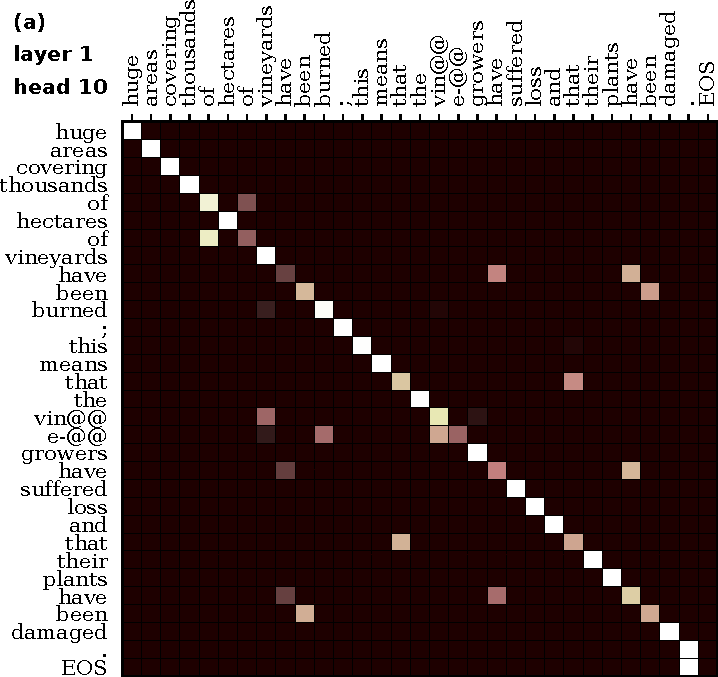
\includegraphics[width=0.5\textwidth]{balustrades/hms3-n-k9-l0-e.pdf}\hspace{2mm}
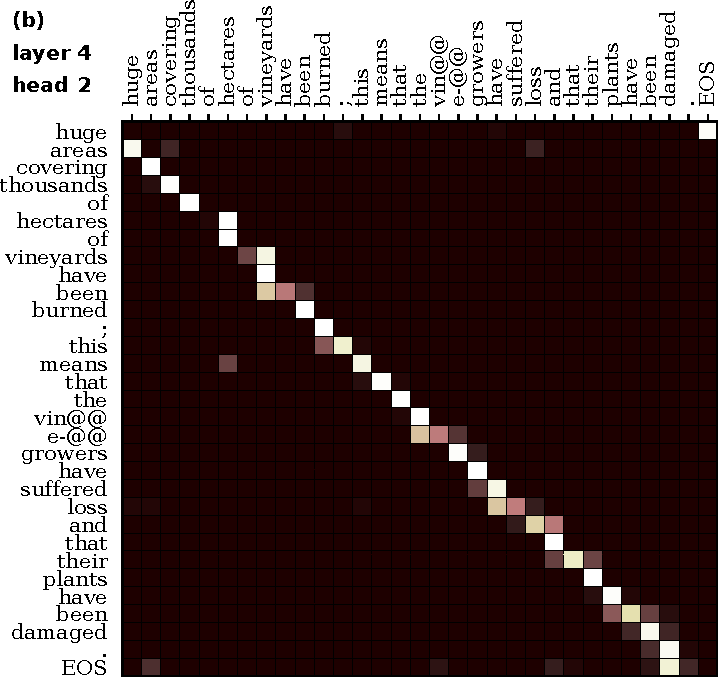
\includegraphics[width=0.5\textwidth]{balustrades/hms3-n-k4-l0-e.pdf}\\
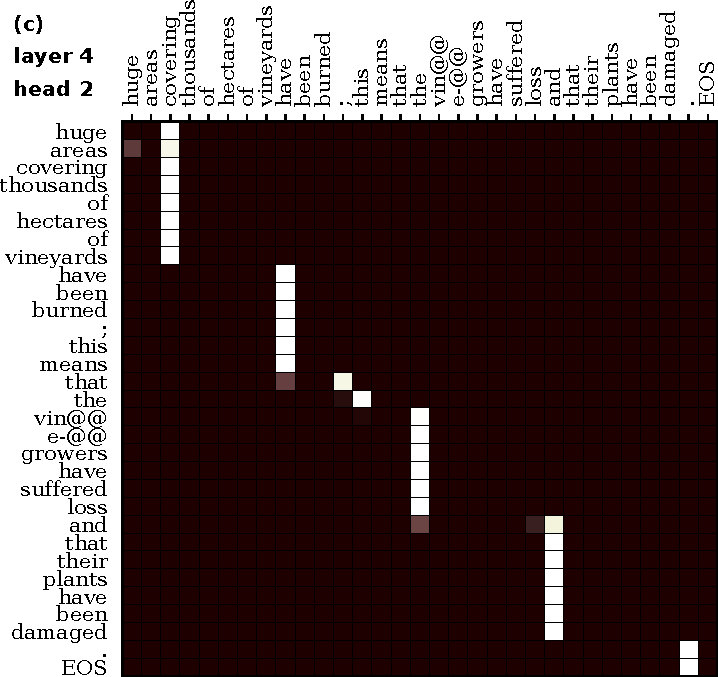
\includegraphics[width=0.5\textwidth]{balustrades/hms3-n-k1-l3-e.pdf}\hspace{2mm}
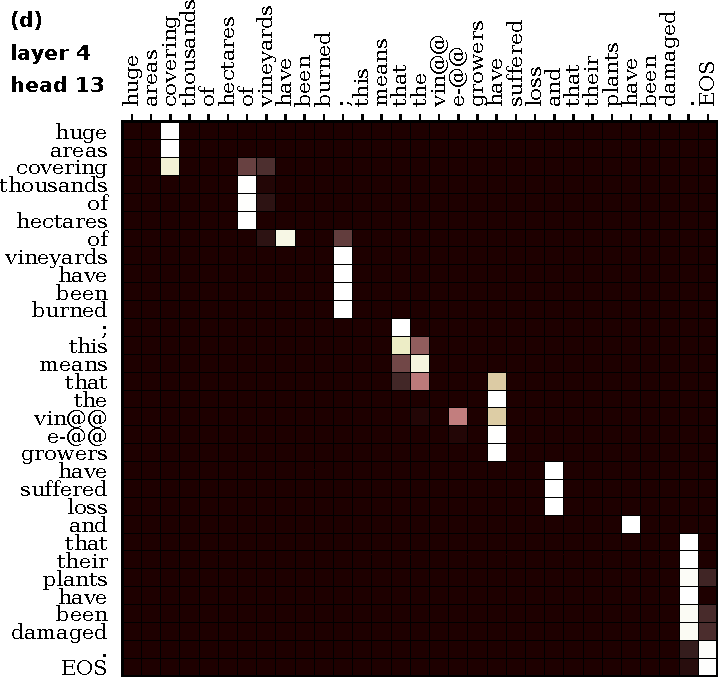
\includegraphics[width=0.5\textwidth]{balustrades/hms3-n-k12-l3-e.pdf}\\
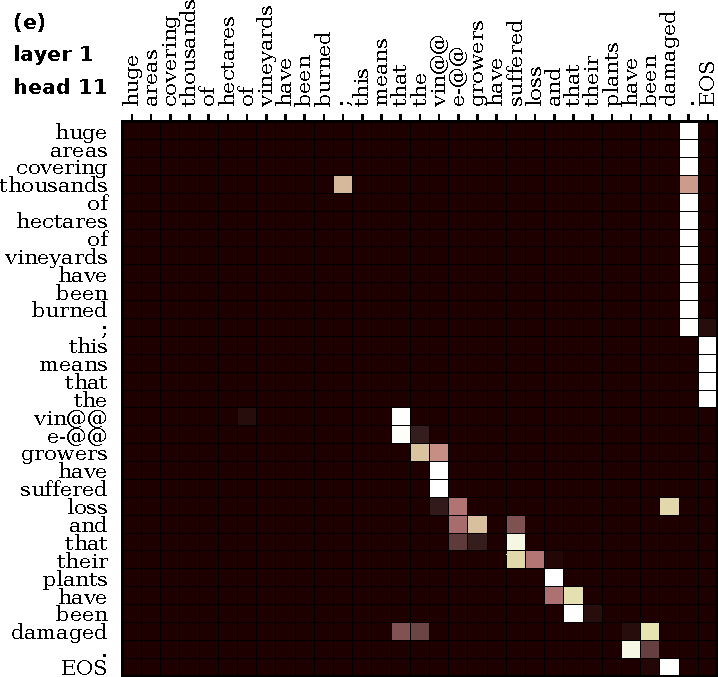
\includegraphics[width=0.5\textwidth]{balustrades/hms3-n-k10-l0-e.pdf}\hspace{2mm}
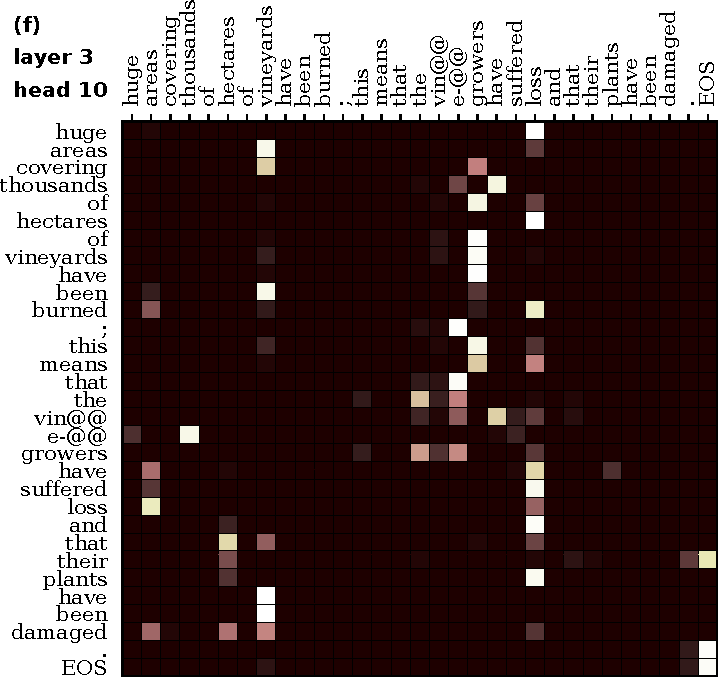
\includegraphics[width=0.5\textwidth]{balustrades/hms3-n-k9-l2-e.pdf}\\
\caption{Heatmaps of selected attention heads showing different patterns.
There are \emph{diagonal} patterns in (a) and (b), \emph{balustrades} in (c) and (d), a combination in (e), and rather scattered attention in (f).}
\label{fig:heatmaps}
\end{figure*}

%\begin{description}
%\item[\word] is the hidden state from the previous layer, that the head may attend to
%\item[\state] is the hidden state on this layer, composed of the words that the head attends to (plus residual connection)
%\end{description}

%Možnosti: attended, attending. Input word, output word. Input state, output state. Word, head. Input, output.

A general observation is that the attentions are nearly always very peaked. Even though the attention mechanism was designed as soft, most attention heads concentrate nearly all of the attention at each \state onto just one \word.
%The exception is the German-French language pair, where we observe much softer attentions.
%\DM{TODO FIGURE OF DE-FR GHOSTS?}
%\JL{takhle už to bylo i v případě klasickýho attentionu, tak by to nemuselo bejt takový překvapení}
%\RR{This leads us to believe that summing up representations of several \words together is not very useful for the system -- representing a phrase or the full sentence by a simple weighted average is probably a too crude PŘEDPOTOPNÍ, DŘEVNÍ way, resulting in a difficult-to-use representation.}
%The encoder seems to strongly prefer attending to each of the relevant \words in separate heads and then obtaining the combined representation by concatenation \RR{rather than averaging}.\JL{jenže ten averaging se děje hned za tou konkatenací}

%We identify several patterns that we frequently observe in the heatmaps.
In the following subsections, we list all of the distinctive patterns that we have identified.\footnote{%
We observe all patterns which \citet{raganato:2018} identified, i.e.\ diagonals and attending to the end of the sentence, but also other patterns which they did not observe.}
%\DEL{in the attention heatmaps}.
An important thing to note is that typically, a head behaves consistently across all sentences, i.e., for a given head on a given layer of a given trained Transformer encoder, we typically see the same attention patterns across all sentences.

%\RR{Srovnání sTidemanem?}

% \DM{Analysis of attentions combining the \words across all heads is left for the future research.}
% \RR{To nevim co se tim myslí ani proč to tu je.}

\subsection{Diagonals}

Especially at the first encoder layer, there often appear various simple \emph{diagonal} heads.

Typically, each \state attends to the \word at the same position.
%\DEL{We call them a \emph{full diagonal}.}
This may serve
%Their role may be
to pass the subword information to the higher layers.

In some cases, most of the \states attend to the corresponding \words, but some of them attend elsewhere. The role of such \emph{partial diagonal} may be looking for a specific phenomenon that only occurs for some of the \states.
%; for the other \states, the head may be ``parked'' at the diagonal.
%Attending to the diagonal is just a way of ``parking'' the head when the phenomenon is not relevant or present for the given \state. \JL{nechápu, co je parking}

%In many cases,
Often,
individual \states attend to preceding or following \words, forming a \emph{parallel diagonal} (Figure~\ref{fig:heatmaps}b).
%The two most common placements of this parallel diagonal are:
%\begin{itemize}
%\item just above the diagonal: the \word is the word immediately following the \state.
%\item just below the diagonal: the \word is the word immediately preceding the \state.
%\end{itemize}
Sometimes the heads attend further, \eg to the ``pre-previous'' \word.
%Such heads are also mostly present at the first layer.

% \RR{\subsection{Watching the end}
% Attending to the sentence-final dot \DM{full stop?} (or other \JL{punctuation} mark).
% A long vertical bar in the penultimate column, spanning most or all of the words.
% %
% Hypothesis 1: The lower layers may concentrate information about the whole sentence into the sentence-final \JLrepl{dot}{punctuation}, so a fixed-size sentence representation may be stored here.}
% %
% \RR{Hypothesis 2: A parking space for the attention head when there is nothing interesting to attend to for the given position, similarly to the partial diagonal.
% %
% Hypothesis 3: The sentence-final punctuation mark indicates the sentence mood (indicative, imperative or interrogative).
% %
% As the vast majority of sentences in our dataset are indicative, we find the hypothesis number 3 rather unlikely.
% In case of hypothesis 2, we see no clear reason why the head would attend to the sentence-final mark (which may differ and may not always be there) and not to the ``EOS'' symbol (which is fixed and always there).
% This may suggest hypothesis 1 as the most plausible, but we have yet to test this.\footnote{The future work is clear: evaluate the final encoder \states using a sentence representation evaluation, such as SentEval CITE, and see whether some of the \states seem to represent the whole sentence better than others. Our hypothesis is that sentence-final punctuation \state represents the whole sentence best, while linking tokens \states such as other punctuation and conjunctions represent larger parts of the sentence.}}
% \JL{Tohle by se mělo udělat buď pořádně nebo bych to vůbec nezmiňoval. Jestli masáž článku je, že umíte měřit, skladebnost sebepozorností, tak tohle je navíc.}

\subsection{Balustrades}

The most frequent pattern, appearing in about 2/3 of the attention heads, are \emph{balustrades} -- a series of vertical bars, typically placed at the diagonal, which resemble the balusters of a staircase railing.
Examples of such balustrades are shown in Figure~\ref{fig:heatmaps}c,d,e.
The balustrades are often placed upwards or downwards from the main diagonal.
\DEL{Sometimes they are crossing it or floating somewhere else.}

%The balustrades can be placed in the following ways, in relation to the diagonal:
%\begin{description}
%\item[upward] the bottom of the baluster is at the diagonal REF FIGURE; frequent
%\item[downward] the top of the baluster is at the diagonal REF FIGURE; frequent
%\item[floating upward] the baluster is above the diagonal but does not touch it REF FIGURE; less frequent
%\item[floating downward] the baluster is below the diagonal but does not touch it REF FIGURE; less frequent
%\item[crossing] the baluster crosses the diagonal REF FIGURE; rare
%\end{description}
%Usually, a head contains either upward or downward balusters, not both.

%A baluster is formed when a consecutive sequence of \states all attend to the same \word, \eg because the network decides to generate similar \emph{Query} vectors for all of these \states.
%This probably happens when the dot-product attention generates similar Queries for each of the \states.
%It is important to understand that while a baluster appears as a distinctive feature, it is in fact created independently, as the attention is computed independently for each position of the head, so there is no decision of the network to create the baluster, but rather a set of independent decisions to create each of the bright points that eventually end up forming a baluster.
%It is thus quite interesting that the balusters are so frequent.
%On the other hand, 
%\JL{S tou nezávislostí bych to neviděl tak silně. Keys vznikají nějakou projekcí z toho předchozího stavu. Balustráda pak vznikne tehdy, slova v balustrádě touhletou projekcí zobrazí na něco podobného. Ta projekce vyndá ze stavu nějaký druh informace, a protože má k dispozici informaci o poloze, tak může naschával dělat sousedy podobnější a podoporovat balutrádovitost. QUERY MŮŽE BEJT STEJNEJ PRO NĚKOLIK NMÁSLEDUJÍCÍCH INSTAVŮ TAKŽE PAK VYBEROU TEN SAMEJ KEY}

We observe that different heads contain balusters of different lengths. 
For longer balusters, the \word that they attend to often corresponds to a punctuation or a conjunction; often there are also heads that attend exclusively or almost exclusively to the sentence-final punctuation.
%(comma, dash, colon\ldots) or to a linker word (conjunction, preposition used as conjunction).
%\RR{In case of balusters crossing the diagonal, we hypothesize that the crossing point (\ie the \word attended to) might correspond to a head of the phrase.}\JL{Buď to ověř nebo nehypozézuj.}

We have noticed that in many cases, the sequence of subwords spanned by a baluster may be understood as a syntactic phrase (\eg a noun and its determiner, or a syntactic clause between two commas).
Furthermore, by looking at multiple attention heads at once, we can interpret the balusters of various lengths spanning the same subwords as shorter phrases nested within longer phrases.
This leads us to the idea of constructing a constituency tree from the nested phrases, and comparing it with classical syntactic constituency trees (see Section~\ref{sec:parsing}).

%As the lengths of the balusters vary a lot, it is often the case that a sequence of \words is spanned by a single baluster in one attention head, and by a sequence of several balusters in another head. This may be viewed as nested phrases.

%\RR{For us, balusters are most intriguing, as they seem to somewhat correspond to \JL{constituency?} syntactic phrases. Our interpretation of balusters is that typically, the sequence of \states all attend to a \word which forms a boundary of the phrase -- either at its beginning (downward baluster) or end (upward baluster). We may thus extract a syntactic phrase from the attention matrix as a continuous sequence of \states that all attend to the same \word. In this case, we do not really care what they attend to; we hypothesize that the hidden state corresponding to the phrase boundary may represent the whole phrase, but we have not tested that.}

%\RR{Furthermore, we observed that different heads contain balusters of different lengths. This naturally leads to the idea of the longer balusters representing longer phrases, and the shorter balusters their subphrases. Once we have the notion of longer phrases composed of shorter subphrases, we are ready to use this interpretation to build constituency syntax trees from the self-attentive matrices, without the need of using any other information.}

%\RR{Some balusters are torn apart -- there is a baluster, then one or two black squares, and then it continues. Currently, we treat this as two independent balusters. Other possible interpretation: gapped phrases.}

%\RR{The self-attentions are really good at identifying longer phrases bordered by clear connector tokens (commas, dash, conjunction). For shorter phrases, it is less clear what the attentions do...}\JL{tohle by taky šlo kvantifikovat}

%\JL{Další kvantitativní ukazatel, co by vám pomohl podpořit hypotézu o balustrech by bylo spočítat, jak často balustr končí uprostřed slova rozděleného na subwordy.}


\subsection{Equal or Similar Subwords}
There is typically one or two heads where each \state attends to all instances of the same subword, usually with a more or less uniform distribution (see the subwords ``of'', ``have'' and ``that'' in Figure~\ref{fig:heatmaps}a).
%For most words, this simply means attending to the diagonal.
%However, in most sentences, there are repeated tokens, at least determiners (``a'', ``the''), and often also prepositions, conjunctions or auxiliaries.
\RR{Hypothesis: position-independent word identity (like a bag of words).}
%
We have also seen these heads to sometimes attend to very similar but not identical subwords (\eg singular and plural).
%, which probably have very similar embeddings.
%most probably due to their word embeddings being very similar.
%and thus hard to distinguish for the self-attentive mechanism.
% \RR{However, we have not noticed any case of attending to less similar words (\eg synonyms, hyperonyms, deverbative nouns, etc.), which are typically also quite similar in the embedding space and would thus presumably be easy to attend to.
% We thus hypothesize that the attention heads are not trying to attend to similar words; they are only trying to attend to identical words, and the occasional attention to a similar but non-identical word is simply an artifact of the word embeddings.}\JL{tohle by platilo, kdyby tam nebyly ty projekce do hlav, s projekcema do hlav je to celý pak zašmodrchanější}\JL{tohle by šlo spočítat, jak často se to děje}

\DEL{\subsection{Not Peaked}
Quite rarely, we see heads that are not as peaked, distributing the attention over multiple \words, usually consecutive or close to each other.
We believe that this is simply a way of obtaining a representation of a whole phrase, but we do not have any explanation for why this happens in some cases.
We frequently observe such heads only in the German-to-French translation pair.
%; in most cases this does not happen, as we already noted and explained at the beginning of this subsection.
}

%\JL{tohle by taky možná šlo kvantifikovat tu vypíkovanost, třeba počítáním entropie na těch distribucích}

\subsection{The Rest}

Admittedly, for about 1/5 of the attention heads, we have not identified any clear pattern, and thus have no hypothesis as for the function of such heads.
%They can simply be described as not belonging to any of the aforementioned types. 
Sometimes, the head shows some of the behaviours only for some of the \states; sometimes we do not see even such partial patterns (Figure~\ref{fig:heatmaps}f).
% \RR{They may be performing a function that we have not thought of and thus have been unable to identify.
% Or, they may simply not be susceptible to the kind of analysis we are performing. For example, they may ignore the information in the representations relating to the source subwords, and rather use the available ``memory'' to store some global information. While the residual connections strongly discourage this, the architecture encompassing several layers of self-attentions and fully connected network layers is powerful enough to delete or ignore the information about the source tokens.}

%\subsection{Quantitative evaluation}
\DM{TODO: Quantitative evaluation: try to say how many patterns of type X are present for lang pair Y-Z
(and potentially also try to interpret this)}

\section{Extracting Constituency Trees}
\label{sec:parsing}

%\begin{figure}
%\begin{center}
%\includegraphics[width=0.5\textwidth]{hms5-n-k10-l2-phrases.pdf}
%\end{center}
%\label{fig:phrases}
%\caption{Extracted phrases.}
%\end{figure}

Our aim is to analyze whether syntactic structures seem to be captured by Transformer self-attentions, to what extent, and of what kind.
As explained in the previous section, we often observe balusters of various lengths in the attention heatmaps, which can be interpreted as nested syntactic phrases.
In this section, we try to measure
%and analyze
to which extent this interpretation seems to be valid.

For this purpose, we devise a linguistically uninformed transparent deterministic algorithm to extract binary constituency trees from the balusters (Section~\ref{sec:algorithm}).
We automatically evaluate the results by comparing them with classical syntactic trees, generated by a standard syntactic parser (Section~\ref{sec:eval}), to see whether the observed structures seem to capture syntax as we know it.
We discuss the results in Section~\ref{sec:results}.

%, a logical approach is to utilize them to build constituency trees, and see whether they seem to represent the syntactic structure of the sentences.

%While building a constituency tree may seem as a linguistically informed process, we believe that a binary constituency tree is the simplest possible way of representing a set of nested phrases.

%From our analyses, it is evident that the attention heads frequently form balusters, \ie sequences of consecutive \states attending to the same \word, of various lengths.
%Furthermore, we have noted that the balusters often resemble syntactic phrases.

\subsection{Tree Extraction Algorithm}
\label{sec:algorithm}

%Our aim is to extract candidate phrases from the attention matrices, and try to build constituency trees from them.\footnote{A constituency tree seems to be the most logical and uninformed way of representing a set of shorter and longer phrases.}

%\RR{Standpoint:}
%We do not optimize towards good trees. Our only goal is to analyze what the attentions do, what kind of syntactic structures they seem to capture and in what ways. We thus devise a deterministic tree extraction algorithm that is as linguistically uninformed as possible, only making use of the fact that we can extract phrases from the attentions, not \eg tuning any hyperparameters to obtain good syntactic trees.

%Our aim is to extract such sequences and use them as phrases for building constituency trees.

We now explain how we construct constituency trees from the balusters in the attention matrices.

Our goal is not to optimize our algorithm towards producing good syntactic trees. Rather, we try to keep our algorithm linguistically uninformed, to reveal only what really is captured by the self-attentions.
%For this reason,
Therefore, we:
\begin{compactitem}
\item build binary constituency trees, as this is quite a
%very simple and logical
%very
basic
way to represent nested phrases,
\item use information from all attention heads, not only those which seem to capture syntax,
%contain syntactic information,
\item keep the number of other hyperparameters minimal and set them to the most uninformed values, rather than tuning them,
\item do not train or tune the tree extraction in any way (unlike most related work).
\end{compactitem}

The first step is to identify the balusters.
We have previously described a baluster as a sequence of \states attending to a single \word.
The attentions are typically very peaked, with nearly all of the attention mass concentrated onto one \word.
However, as the attentions are soft, each of the \states in fact attends to all of the \words to some extent.
We thus ``harden'' the soft attention matrix $A'$ by only keeping the maximal attention weight on each row of the attention matrix, setting all the other weights to 0:
\DEL{(see also Figure~\ref{fig:line}):}
%\RR{Možná stačí vzoreček, obrázek lze smazat?}
\begin{equation}
A_{o, i} = \begin{cases} A'_{o, i} & \text{if } A'_{o, i} = \max_{j \in [1,N]} A'_{o, j}\\
0 & \text{otherwise}\end{cases}
\end{equation}
where $i$ is the \word index, $o$ is the \state index,
%$A'$ is the original attention matrix, $A$ is the hardened attention matrix,
and $N$ is the sentence length.

\DEL{
\begin{figure}
\begin{center}
\includegraphics[]{balustrades/line}
\end{center}
\caption{Hardening the attention on one row.}
\label{fig:line}
\end{figure}
}

%Some phrases are clear (all their \states attend to a single \word), but some are not as clear and it is often hard to recognize their beginnings and ends.
%To exactly determine phrases, we simply take the maximum instead of softmax for each \state (row in the heatmap matrix).
%\DM{JE NUTNY OBRAZEK< NEBO JE TO JASNY?}\JL{obrázek}
%\RR{obrázek: původní řádek heatmapy, a pak ten samej řádek kde maxium je ponechaný a ostatní buňky jsou černý (ale maximum si zachovává svojí váhu, tj. neni bílý)}

Next, we extract candidate phrases from the balusters and weight them.
From each baluster, we extract only the candidate phrase corresponding to the full length of the baluster.
%Each candidate phrase of the source sentence is scored.
The weight of the phrase corresponds to the average attention that \states in the phrase give to the common \word they attend to (\ie the average brightness of the points in the baluster).
If the same phrase appears in multiple attention matrices,
%which is especially frequent for shorter phrases,
%(and for the shorter phrases, they often do),
their scores are summed together.
The weight of the phrase spanning the $a$-th to $b$-th subwords thus is:
\begin{equation}
w'_{a,b} = \sum_{h \in H_{a,b}} \frac{\sum_{o \in [a, b]} A^h_{o, i_h}}{b - a + 1}
\end{equation}
%\DM{Tady to $i$ je takovy spadly z nebe. Je to pozice toho balustru v hlave h.}
%\RR{$i$ se definovalo už u předchozí equation. Ale může se tu definice zopakovat, ať je to jasné.}
where $H_{a,b}$ is the set of attention heads containing a baluster
spanning the \states $a$ to $b$,
%starting at the $a$-th and ending at the $b$-th \state,
$A^h$ is the hardened attention matrix for head $h$, and $i_h$ is the \word attended by the baluster in head $h$.

The weights defined in this way are unbalanced, giving more importance to shorter phrases, as they are more frequent in the attention matrices.
%being higher for shorter phrases, as they often appear in multiple attention matrices.
We thus equalize the weights so that the average weight of all phrases of the same length equals 1:
\begin{equation}
w_{a, b} =  \frac{w'_{a, b} \cdot |P^{b-a+1}|}{\sum_{(c, d) \in P^{b-a+1}} w'_{c, d}}
\end{equation}
where $P^k$ is the index pair set of all extracted phrases of length $k$.

% not equalized: short phrases have a too high weight (hodně binární stromy)
% normalized to form a distro: long phrases have a too high weight (branching degeneration, pagody)

%\JLrepl{It is evident that t}{T}he often repeating \JL{of} shorter phrases would get much higher weights than the longer ones and therefore we normalization\JL{?}, so that the average weight of all phrases with the same length must equal to one.

\DM{Example of visualized phrase weights is given in Figure
TODO: vizualizace vah kandidatskych frazi.}

%\RR{Now, joining two shorter phrases to form a longer phrase is as good as the two smaller phrases + the longer phrase. Avoiding any hyperparameters -- shorter and longer phrases weighted equally, only binary trees...}\JL{Tuhle větu IMHO napsal kapitán obvous.}

To construct the constituency tree from the phrases,
we use the CKY dynamic programming algorithm~\cite{ney:1991}, which searches for the highest scoring constituency tree in $O(n^3)$.
%It is a bottom-up parser using a dynamic programming table.
%To minimize the amount of hyperparameters used, we generate strictly binary trees, \ie each phrase is divided into two subphrases (unless it as a terminal phrase, representing a single subword).
%...already noted at start of section

For each tree spanning the $a$-th to $b$-th subword, we define its score $s_{a, b}$ recursively by
finding a separator $k$, $a \le k < b$, that maximizes the average of scores and weights of the two subtrees with spans $(a, k)$ and $(k+1,b)$:
%
%For the algorithm, we define the score $s_{a, b}$ of a tree spanning the $a$-th to $b$-th subword recursively by maximizing the \emph{score} of its two subtrees:
%\begin{equation}
%v_{a, b} = \begin{cases} 1 & \text{if } a = b\\
%\max_{k, a \le k < b} s_{a,k,b} & \text{otherwise}\end{cases}
%s_{a,a} = 1
%\end{equation}
\begin{equation}
s_{a,b} = \max\limits_{k} \frac{s_{a,k} + s_{k+1,b} + w_{a,k} + w_{k+1,b}}{4}.% \text{otherwise}
\label{eq:value}
\end{equation}
%
%where $s_{a, k, b}$ is the \emph{score} of a pair of trees,
%the first one
%spanning the $a$-th to $k$-th subword and
%the second one spanning
%the $(k+1)$-th to $b$-th subword, defined recursively by averaging the \emph{values} of the trees and the weights of the phrases spanning the same subwords:
%
%\begin{equation}
%s_{a, k, b} = \frac{v_{a,k} + v_{k+1,b} + w_{a,k} + w_{k+1,b}}{4}
%\label{eq:score}
%\end{equation}
The initial scores for single-subword subtrees are set to 1.
The averaging then keeps the scores equalized -- subtrees then have the same power regardless of the size of their spans.
%\RR{(\ref{eq:value}) a (\ref{eq:score}) lze zmergovat, a zkrátit popis.}

The CKY algorithm works bottom up, starting with the trivial single-subword trees, and then iteratively computing the values of larger subtrees based on the values precomputed in previous steps. Together with the score of each tree, the algorithm also stores the $k$ from Equation~\ref{eq:value}, which defines the highest scoring pair of subtrees covering the same span.
Once the algorithm reaches the tree covering the whole sentence, it recursively returns the highest scoring tree based on the stored values of the highest scoring subtrees.

\RR{Tady je zakomentovanej původní popis, ten můj mi přijde lepší, ale asi taky neni dokonalej, a nejlepší by byl nějakej merge těch dvou.}

%The algorithm proceeds as follows:
%The scores of the phrases with span 1 (individual words) are initialized by 1. Scores of phrases with higher spans are then dynamically computed using already precomputed scores of shorter phrases and their weights.
%For each phrase $(i,j)$, we find such separator $k$ between $i$ and $j$ that maximizes the scores and weights of the two subphrases $(i, k)$ and $(k+1,j)$. \begin{multline}
%score(i,j) = \frac{1}{4}\max_k(score(i,k) + w(i,k) +\\+ score(k+1,j) + w(k+1,j)),
%\end{multline}
%where the weights $w$ are the phrase weights computed from the attention matrices, while the scores are already aggregated weights of the whole subtrees.
%In each step, we \JLrepl{make}{compute} the average of the four values (two weights and two scores).
%All of them are distributed with the mean equaling 1, so the resulting score should also keep it.
%Therefore, when joining two phrases, scores of their subtrees have the same power as their weights obtained from the self-attentions. We do not tune these weights so that our approach is as uninformed and parameter-less as possible.
%\JL{a co děláte se subwordama tady?}

\subsection{Automatic Evaluation}
\label{sec:eval}

To evaluate the syntacticity of the Transformer self-attentive encoder,
we extract the constituency trees using our tree extraction algorithm for the 1,000 sentences of our evaluation set;
\DEL{, using all the 6 translation directions;} we will refer to these as \emph{extracted trees}.

We then induce 
%classical
syntactic trees for these sentences
with the Stanford Parser.
We use the factored lexicalized parsing models distributed together with the parser, which had been trained on standard constituency treebanks of the languages --
English Penn Treebank \citep{penntb},
German Negra Corpus \citep{negra},
and French Treebank \citep{ftb}.
We post-process the trees in the following way:
\begin{compactenum}
\item remove phrase labels
\item wrap each word into a single-word phrase
\item split words into subwords
\item flatten phrases containing only one immediate subphrase or only one subword
%\DM{to tam nastava? Spis bych rekl, ze odstranujeme zpet ty single-word-phrase}
\end{compactenum}
%\begin{compactenum}
%\item remove phrase labels\\
%      \textsl{( (vinegrowers suffer) )}
%\item wrap each word into a single-word phrase\\
%      ( ( (vinegrowers) (suffer) ) )
%\item split words into subwords\\
%      ( ( (vin- e- growers) (suffer) ) )
%\item flatten phrases containing only one subphrase
%      ( (vin- e- growers) suffer)
%\end{compactenum}
We show an example of applying this procedure:
\begin{compactenum}
\setcounter{enumi}{-1}
\item (S (VP vinegrowers suffer) )
\item ( (vinegrowers suffer) )
\item ( ( (vinegrowers) (suffer) ) )
\item ( ( (vin- e- growers) (suffer) ) )
\item ( (vin- e- growers) suffer)
\end{compactenum}
We will refer to the resulting trees as \emph{parse trees}.

\RR{Ta ukázka neni moc hezky formátovaná. Ale myslim si že je vhodný ji tu mít.}

%Each sentence in the test data is parsed also using the Stanford parser \DM{CITACE, URL} obtaining a pseudo-gold parse tree.
%For each sentence in the test data:
%\begin{compactenum}
%    \item We construct constituency tree using CKY parser based on the multi-head self-attentions. Tokens of this tree are the BPE subword units preprocessed by the Stanford tokenizer.
%    \item We parse the sentence using Stanford parser, obtaining a pseudo-gold parse tree.
%\item compute the accuracy of our tree $O$ using the pseudo-gold tree $G$
%\end{compactenum}
%We decided to use pseudo-gold trees on the Europarl test sentences rather than using part of treebanks as testing data, since the domain of the treebanks is different from Europarl\JLrepl{and it was more convenient for us to use easily accessible Stanford parser with all its models and unified output rather than obtaining and converting manually annotated treebanks.}{\ldots to zní jak zbytečná vymlouvání}
%\DM{TODO: co je to za treebanky?}
%TODO ale to je problém i když parsujem Europarl parserem natrénovanym na těch treebankách, a možná tenhle problém je větší; to bychom měli vysvětlit nějak pořádně; navíc když ani nevím jakou accuracy vlastně ten Stanford parser má... Reálnej důvod je že nám přišlo jako moc práce shánět ty treebanky a srát se s konverzema a tak, zatimco Stanford parser umí parsovat všechny tyhle jazyky a výstup plive pro všechny ve stejnym formátu... Aspoň za mě (RR) je tohle ten důvod.

We compare the extracted trees with the parse trees, assuming that the more similar they are, the more syntactic the Transformer encoder is.

%We evaluate the extracted trees using the crossing brackets ratio.
%The constituency trees are expressed in a bracketed way, where each phrase is enclosed in brackets,
%ignoring the phrase labels (\ie the non-terminal symbols).
%We remove brackets containing only one member (such as a noun phrase containing only one noun, which may appear in the gold trees).
%We also need to handle the words that are split into subwords (although most words are unsplit in our data, so this step is not crucial).  For each split word, we add a gold phrase consisting only of the subwords that form that word.

%\RR{TODO But some of the baselines may suffer, we might want to make them even stronger by keeping the split words together in the baselines.}

%\RR{TODO: maybe we should first somewhow binarize the stabdard trees? Chmosky NF or sth like that? Now they often contain flatter phrases, composed directly of more than 2 phrases.}

%We then evaluate the trees by counting ``crossing brackets''.
We calculate the \emph{precision} of the extracted tree as the proportion of its phrases that are ``correct'' in the sense that they are consistent with the parse tree,
not crossing any of its phrases.
% based on the notion of crossing brackets.
\DEL{An extracted phrase is correct if, for each phrase in the parse tree, one of the phrases is contained in the other, or they are disjoint; \ie,}
%Otherwise, \ie if the extracted tree phrase intersects with a phrase in the parse tree but none of them is contained in the other, it is counted as incorrect.
(For the sake of this analysis, we only consider one possible way of capturing syntax, as defined in the respective treebanks; we
%get back to this issue
discuss that
in Section~\ref{sec:results}.)

Let $P$ be the parse tree, an extracted phrase $e$ is correct if and only if:
\begin{equation}
\forall p \in P: (p \cap e = \emptyset) \vee (p \subseteq e) \vee (e \subseteq p).
\end{equation}

%A phrase in the extracted tree is evaluated as correct if it does not cross any of the phrases in the parse tree. For each of the pseudo-gold phrases that have a non-empty intersection with our phrase, we check whether they are identical, or whether one contains the other. If so, the phrase is correct, as it is consistent with the pseudo-gold parse tree.
%Otherwise, the phrase is not consistent with the parse tree and is evaluated as incorrect.
%We denote the ratio of correct phrases as the precision of our tree.
\emph{Recall} is computed inversely, as the proportion of phrases in the parse tree that are consistent with the extracted tree.
We compute the total precision and recall as an average over all extracted phrases in all the trees\DEL{ (\ie not as a macro average over the sentences)},
and also report their harmonic mean (\emph{F1}).
%We also compute the harmonic mean of the precision and recall, denoted as \emph{F1}.


The results of the evaluations for all three source languages are shown in Table~\ref{tab:results}.
To put them into perspective, we also report scores for several uninformed parsing baselines:
%We also compute the scores for the following four baselines:
\begin{compactenum}
%\item \emph{rbr}: right-branching tree
%\item \emph{lbr}: left-branching tree
\item \emph{rbal}: balanced binary tree aligned right
\item \emph{lbal}: balanced binary tree aligned left
\item \emph{rand.init}: our proposed algorithm using randomly initialized Transformer weights
\end{compactenum}
Examples of the \emph{lbal} and \emph{rbal} baselines are shown in Figure~\ref{fig:baselines}.
%\RR{Vysvětlit co znamená která baseline? Řiká se tomu balancovanýmu stromu nějak?}

\begin{figure}[t]
\begin{center}
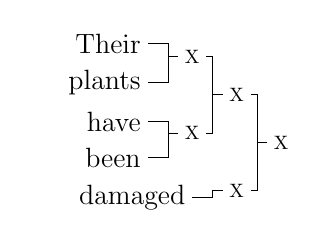
\begin{tikzpicture}[scale=0.7, grow=left]
\tikzset{every leaf node/.style={font=\Large, align=right, anchor=east, text width=55pt}}
\tikzset{level distance=23pt}
\tikzset{edge from parent/.style=
{draw,
edge from parent path={(\tikzparentnode.west)
-- +(-5pt, 0)
|- (\tikzchildnode.east)}}}
%\tikzset{sibling distance=5pt}
%\LARGE
\Tree
  [.X
    [.X
      [.X Their plants ]
      [.X have been ]
    ]
  [.X damaged ] ]
\end{tikzpicture}
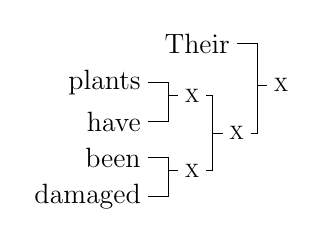
\begin{tikzpicture}[scale=0.7, grow=left]
\tikzset{every leaf node/.style={font=\Large, align=right, anchor=east, text width=55pt}}
\tikzset{level distance=23pt}
\tikzset{edge from parent/.style=
{draw,
edge from parent path={(\tikzparentnode.west)
-- +(-5pt, 0)
|- (\tikzchildnode.east)}}}
\Tree
  [.X Their
    [.X
      [.X plants have ]
      [.X been damaged ]
    ] ]
\end{tikzpicture}
\end{center}
\caption{Left (\emph{lbal}) and right (\emph{rbal}) balanced binary tree baselines.}
\label{fig:baselines}
\end{figure}


%\DM{parseval?}
%\DM{TODO the rest only if we also include the special eval}

%\DM{additional eval: remove pucntuation, eval only on sentences of max 10 tokens. This makes rbr strong for English, as without punctuation (which is annotated in a special way), the PennTB is mostly right branching...}

%\DM{eval on 100? 1000? test sentences -- standard eval on first 100 sentences, nopunct max10 eval on all 1000 sentences (but the max10 filter reduces the number to only about 100 sentences anyway)}


\subsection{Discussion of Results}
\label{sec:results}


\begin{table}[t]
\centering
\emph{English}
\begin{tabular}{l|rrr}
system & precision & recall & F1 score \\
\hline
%rbr      & 15.2\% &	11.0\%	& 12.7\% \\
%lrb      & 15.6\% &	9.7\%	& 12.0\% \\
rbal     & 30.1\% & 24.3\%	& 26.8\% \\
lbal     & 27.8\% &	20.8\%	& 23.8\% \\
rand.init& 25.1\% &	20.0\%	&22.3\% \\
\hline
en $\rightarrow$ de & 35.4\% & 30.6\% & 32.8\% \\
en $\rightarrow$ fr & 35.4\% & 30.2\% & 32.6\% \\
\end{tabular}
\medskip

\emph{German}
\begin{tabular}{l|rrr}
system & precision & recall & F1 score \\
\hline
%rbr      & 21.3\% & 16.7\% & 18.8\% \\
%lbr      & 23.4\% & 14.1\% & 17.6\% \\
rbal     & 39.1\% & 31.3\% & 34.8\% \\
lbal     & 38.1\% & 27.6\% & 32.0\% \\
rand.init& 33.7\% &	25.9\% & 29.3\% \\
\hline
de $\rightarrow$ en & 46.1\% & 39.6\% & 42.6\% \\
de $\rightarrow$ fr & 46.7\% & 40.9\% & 43.6\% \\
\end{tabular}
\medskip

\emph{French}
\begin{tabular}{l|rrr}
system & precision & recall & F1 score \\
\hline
%rbr      & 19.4\% & 12.2\%	& 15.0\% \\
%lrb      & 21.0\% & 11.6\%	& 14.9\% \\
rbal     & 34.3\% & 28.7\%	& 31.3\% \\
lbal     & 32.5\% & 25.4\%	& 28.5\% \\
rand.init& 26.1\% & 24.4\%	& 25.3\% \\
\hline
fr $\rightarrow$ en & 44.4\% & 39.7\% & 41.9\% \\
fr $\rightarrow$ de & 46.9\% & 41.7\% & 44.2\% \\
\end{tabular}
%\caption{Non-crossing-brackets scores of the trees extracted from the self-attention matrices compared to baselines.
\caption{Scores of baseline trees and our extracted trees using all attention heads, evaluated against standard syntactic parse trees.}
%, evaluated against standard syntactic parse trees.
%\JL{použijte booktabs, bude to vypadat přehleněji; smazat procento ať je to čistší}
\label{tab:results}
\end{table}

The F1 scores of the trees extracted from the attention matrices are 6 to 13 percentage points higher than the best baselines, showing that some syntax
%seems to be
is
indeed captured by the Transformer encoder.

For English, the scores are notably lower than for the other languages.
Manual inspection has shown that this is mostly due to the English parse trees being strongly right-branching, while the other treebanks use flatter, more balanced trees, mainly due to different annotation styles of the treebanks.
The trees extracted from the attention matrices are similar for all of the languages, and resemble the German or French parse trees more than the English ones.
However, a part of the score differences may also be due to a differing syntacticity of the individual encoders, as can be seen from the differing scores for fr$\rightarrow$en and fr$\rightarrow$de.

%The English trees do not look like the . PennTB has strongly right-branching trees, as can be seen from the high score of the right-branching baseline.
%\RR{(especially when ignoring punctuation, since sentence-final dot is not right-branched in PennTB).}
%The trees we get are flatter and more balanced than PennTB trees.

%We can see higher scores for German and French. For these languages, the standard trees obtained by Stanford parser are much flatter and more balanced than the English PennTB-style ones.

%Generally, the trees we get look similarly for all of the languages. So the differences in the scores are probably both due to different styles used in the classical treebanks for these languages, as well as due to the encoders showing a larger or smaller amount of syntacticity for different language pairs.

%We can thus conclude that the encoder does show some syntactic behaviour, \ie that the baluster structures do often correspond to classical phrases.
%Furthermore, we can conclude that this syntax most resembles the style of the Negra German treebank, which had been used to train the Stanford parser for German, and does not resemble much the PennTB strongly right-branching style.

\begin{figure}[t]
%\begin{center}
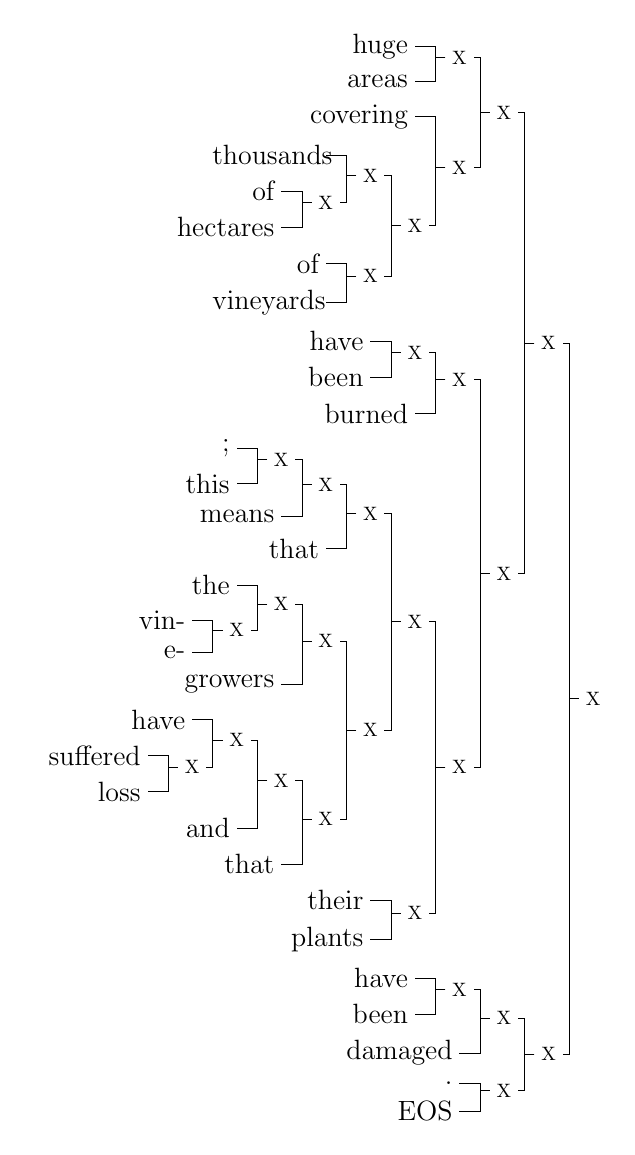
\begin{tikzpicture}[scale=0.7, grow=left]
\tikzset{every leaf node/.style={font=\Large, align=right, anchor=east, text width=55pt}}
\tikzset{level distance=23pt}
\tikzset{edge from parent/.style=
{draw,
edge from parent path={(\tikzparentnode.west)
-- +(-5pt, 0)
|- (\tikzchildnode.east)}}}
%\tikzset{sibling distance=5pt}
%\LARGE
\Tree
[.X
  [.X
    [.X
      [.X huge areas ]
      [.X covering [.X [.X thousands [.X of hectares ] ] [.X of vineyards ] ] ] ]
    [.X
      [.X [.X have been ] burned ]
      [.X
        [.X
          [.X [.X [.X ; this ] means ] that ]
          [.X
            [.X [.X the [.X vin- e- ] ] growers ]
            [.X [.X [.X have [.X suffered loss ] ] and ] that ] ] ]
        [.X their plants ] ] ] ]
  [.X [.X [.X have been ] damaged ] [.X . EOS ] ] ]
\end{tikzpicture}
%\end{center}
\caption{A constituency tree generated by our tree extraction algorithm from the attention matrices of the en-de encoder for the 4th sentence of the evaluation set.
%(The word ``vine-growers'' is split into 3 subwords.)
}
\label{fig:tree}
\end{figure}


Figure~\ref{fig:tree} shows an example of a tree extracted from the en$\rightarrow$de encoder (the sentence is the same as in Figure~\ref{fig:heatmaps}).
We can see that many of the subtrees seem to make sense syntactically, both smaller ones, such as ``[have been] damaged'',
as well as larger ones, such as the tree spanning ``huge\ldots vineyards''.
Some are questionable, but not necessarily wrong, \eg ``[the vine-] growers''.

A clear limitation of our automatic evaluation method is that it only evaluates whether the structures match those of the syntactic formalism of the standard treebank, but it cannot appreciate alternative structures that also make sense syntactically.
However, this issue is hard to solve without a significant amount of manual work.
%\RR{Sbírání/anotace různejch treebanků, nebo nějaký automatický konverze...}

Nevertheless, some structures clearly do not correspond to the syntactic structure of the sentence, regardless of the syntactic formalism that we adhere to. E.g.\ 
the phrases ``their plants'' and ``have been damaged'' belong together, but they are separated in the extracted tree all the way to the root.
The reason we find
%We may see
these incorrect structures in the extracted trees
%due to the fact
may be
that we are using all the encoder attention matrices in the extraction algorithm, even though not all of the attention heads seem to behave syntactically; we investigate this to some extent in the next section.
However, it is also quite likely that the encoder only captures some parts of the syntactic structure of the sentence, not a full syntactic tree
-- especially given the fact that the model is trained to do machine translation, and may thus have no reason to capture structures irrelevant for this task.
%
Moreover, classical syntactic trees are by far not the only possible way of capturing syntax, and it is quite likely that the syntax captured by the self-attentive encoder should be understood differently.\footnote{For example, the syntactic structure could be quite flat, with shorter phrases or treelets joined into a linked list, rather than a complex tree structure with long-distance relations.
Also, we have noted that connectors, such as punctuation and conjunctions, often seem to be part of both of their neighbouring phrases, which could lead to a formalism using partially overlapping phrases.
We intend to investigate this in future.}

%However, their structure is not always identical to the one used in PennTB, and they may thus be evaluated as incorrect in our automatic evaluation -- this is a limitation of our method, but it is not straightforward to solve without a significant amount of manual labour.


%\tikzset{every leaf node/.style={font=\Large, text width=60pt, align=right}}

% zarovnat nody doleva
%\tikzset{frontier/.style={distance from root=250pt}}

%\begin{tikzpicture}[scale=0.7, grow=left]
%\tikzset{every leaf node/.style={font=\Large, align=right, anchor=east, text width=60pt}}
%\tikzset{level distance=22pt}

%\begin{tikzpicture}[scale=0.6, sibling distance=-5pt]

%\tikzset{every node/.style={rotate=90, anchor=north}}
%\tikzset{edge from parent/.style=
%{draw,
%edge from parent path={(\tikzparentnode.west)
%-- (\tikzchildnode.east)}}}


%\subsection{Vague thoughts on Transformer syntax}

% \RR{TODO mixing syntactic theory with annotation style, not sure how to call what where....
% \\
% We have observed that some of the information present in self-attentions is syntactic to some degree.
% The automatic evaluation shows that, when compared to standard constituency trees as produced by the Stanford parser, the trees extracted from the self-attentions resemble the standard trees more than simple baselines.
% \\
% However, the classical treebanks are not the only possible linguistically plausible way of representing the syntactic structure of a sentence. Quite the contrary: a wide range of wildly differing syntactic theories exist, most of which have never been realized in a treebank but stay hidden in books and articles and have only been demonstrated on a handful of example sentences.
% \\
% In our work, we first selected the constituency syntax paradigm rather than the currently more popular dependency one, as the balusters that we observed in the attention heatmaps seemed to strongly resemble phrases, while we have not been able to identify any pattern that would strongly resemble dependency relations (even though we tried).
% Next, we used the most readily available way of automatically evaluating the syntacticity of the representations, by comparing them to standard constituency trees produced by a standard parser.
% \\
% The future work clearly lies in trying to really understand the structures emerging in the attention matrices. It is reasonable to assume that even if the structures are syntactic, they will not closely fit any of the existing theories; it would be extremely surprising if they would closely fit the one theory that we chose to test them against.
% We might either try to look for existing theories that would fit the observed structures, or we can try to construct a theory around our observations.
% \\
% In taking the latter approach, we have come up with several ways the syntactic structures in the self-attentive encoder could be understood (they are partially complementary and partially contradictory):
% \begin{description}
% %
% \item[Chunking.] The simplest is to assume that the encoder only performs chunking, splitting the sentence into a flat list of flat phrases without any complex structure.
% %
% \item[Overlapping phrases.] The fact that the connector tokens (punctuation, conjunctions\ldots) are often attended to by both of the phrases surrounding them could lead to denoting the connectors as belonging to both of the phrases, leading to partially overlapping phrases.
% %
% \item[Linked phrases.] Another option is to say that the connectors belong to neither of the phrases, but rather constitute a different type of element in the structure, linking the phrases -- either forming a flat sequence, or forming a more complex tree superstructure over the phrases.
% %
% \item[Phrase treelets.] There is also some support to see the phrases as having an internal structure. Still, there may or may not be a superstructure over the phrases: the representation could also be a linked list of phrase treelets.
% %
% \end{description}
% }



\section{Selecting Syntactic Heads}
\label{sec:head-selection}
% \RR{vybirani jen nekterejch hlav je podle me tak velkej zasah ze bych tomu dal
% samostatnou subsekci}
% \DM{\begin{itemize}
%     \item nektery hlavy asi nejsou syntakticky, tak zkusime vybrat ty nejsyntaktictejsi
%     \item skore je kupodivu lepsi
%     \item co nam to rika? da se to srovnat s nerizenejma?
%     \item uz jenom jedna hlava je dobra? co dela?
% \end{itemize}}

As we have discussed in Section~\ref{sec:analysis}, there is a range of different types of attention heads.
In our interpretation, some of them, especially the \emph{balustrades}, seem to capture syntactic structures, while others seem not to do so.
A logical step thus is to try to identify the syntactic heads, and only use those for the tree extraction.\footnote{
However, once we start subselecting only some of the heads, we are clearly introducing our expectations about the syntactic structures to be found into the process -- we are now contaminating the so far linguistically uninformed approach with our notion of ``good'' or ``syntactic'' phrases.
}
\DEL{However, there is a big threat hidden in this step.
When using all of the attention heads in the parsing, we truly evaluate what is captured by the heads, without imposing any strong assumptions about the syntax that we want to find in the attentions.
But once we start subselecting only some of the heads, we are clearly introducing our expectations about the syntactic structures to be found into the process -- we are now contaminating the so far linguistically uninformed approach with our notion of ``good'' or ``syntactic'' phrases.
%
This may be wishful thinking, \ie we might be trying so hard to get syntactic trees from the self-attentions as to find stuff that is not really there. There are 96 heads, so it is likely that there is a way of subselecting some of them to increase the parsing accuracy, but we should be careful with the interpretation.
%
2 ways: supervised (evaluate against standard trees), heuristic (define a balustradeness measure and select the most balustrady heads)
%
\subsection{Supervised}
}
%In the supervised approach,

We propose to use the automatic evaluation \DEL{of our parse trees against the standard parse trees} as the criterion for selecting the ``syntactic'' heads. We suggest two greedy approaches: \emph{head addition}, and \emph{head ablation}.

%\RR{Ideálně ty popisy otočit, pač nakonec popužívám head addition, která vychází líp. Případně nechat jen head addition, a říct jen že jsme to zkoušeli i naopak ale bylo to horší.}
In the \emph{head addition} approach, we start with an empty set of heads and then iteratively add the heads one by one, maximizing the precision of the extracted trees in each step, until we have the set of all heads. We then identify the highest scoring head combination that we encountered.

The \emph{head ablation} approach is the logical inverse; we start with all the heads and iteratively remove them until we end up with only one head. 

\DEL{the standard variant of our parsing algorithm, using all of the attention heads to extract phrase scores.
We then try to remove each head, construct the parse trees, and evaluate them against the standard parse trees.
From the evaluated setups, we select the one which achieved the highest score, and iterate, until we end up with only one head.
In each step, we remove the head whose removal leads to the highest increase or lowest decrease of the crossing brackets precision of the resulting tree.
%
The \emph{head addition} approach is the logical inverse of the head ablation approach: we start with no heads, and 
}

\begin{table}[t]
\centering
\begin{tabular}{l|rrr}
& \multicolumn{3}{c}{improvement in} \\
system & precision & recall & F1 score \\
\hline
en $\rightarrow$ de & +9.48\% & +7.01\% & +8.10\% \\
en $\rightarrow$ fr & +8.43\% & +6.23\% & +7.19\% \\
\hline
de $\rightarrow$ en & +4.60\% & +2.06\% & +3.13\% \\
de $\rightarrow$ fr & +5.96\% & +1.76\% & +3.52\% \\
\hline
fr $\rightarrow$ en & +11.58\% & +8.54\% & +9.91\% \\
fr $\rightarrow$ de & +12.16\% & +8.63\% & +10.20\% \\
\end{tabular}
\caption{Evaluation of syntactic heads subselection. Score gains over the base tree extraction as reported in Table~\ref{tab:results}, in percentage points.}
\label{tab:addhead}
\end{table}

We ran the selection algorithms using only the first 100 sentences.
% and computing only the precision
The setups selected as best by the algorithm were then evaluated on the full evaluation set.
%We then evaluated the setups selected as best by the algorithm on the full evaluation set.
As the \emph{head addition} consistently outperformed \emph{head ablation} by approximately 2 percentage points, we only report the evaluation of the \emph{head addition} in Table~\ref{tab:addhead}.

We can see improvements in F1 ranging from 3 to 10 percentage points,
%The results clearly reveal that we optimized for precision.
\DEL{Moreover, the improvements on the 100 development sentences (not shown here) are higher by several percentage points than on the full set.}
%This shows
%the results thus show
showing
that better syntactic trees can be extracted by subselecting the heads.
However, we are perhaps overtuning the setup, and the reported numbers are thus probably somewhat inflated.
Therefore, we are reluctant to draw any strong conclusions from the results.

Nevertheless, the meta-analysis of the heads selected as syntactic is of interest.
For each of the language pairs, between 18 and 32 heads of the total 96 were selected.
However, these are not evenly distributed across the layers.
As we show in Table~\ref{tab:headlayers}, on average, one third of the selected heads come from the first layer, which mostly contains diagonals and short balusters; the last two layers, which contain a lot of balusters of varied lengths, each contributes one fifth of the heads.
%The last layers contain a lot of balustrades, and the selected heads contain balusters of varied lengths, so this is easy to understand.
%However, the first layer mostly contains diagonals, and it is unclear to us how the tree extraction benefits from those.

\begin{table}[t]
\centering
\begin{tabular}{l|cccccc}
L & 1 & 2 & 3 & 4 & 5 & 6 \\
\hline
P & 36\% & 3\% & 10\% & 10\% & 19\% & 21\% \\
\end{tabular}
\caption{Average proportion of attention head layers in the best subselection setups for all language pairs. $L$ is the number of the layer, $P$ is the proportion of the selected heads that come from the given layer.}
\label{tab:headlayers}
\end{table}

%\RR{TODO look at the heads and analyze this properly. But alltogether thats 100 heads, thats too much! The rest is not proper analysis and may not be valid.... Not really identifying syntactic heads. Rather identifies a complementary combination of heads that lead to good parsing. So if there are two similar syntactic heads, only one of them is typically selected because the other one does not bring any new information that would improve the parsing. So there is usually an end-watching head, a parallel diagonal head (phrases of length 2), and then a few heads with balustrades of varying lengths.}

%\RR{Kouklal jsem na ty výsledný stromy (soubory phrases_best_sup_add), a jsou lepší, no. Například ta chyba s tou rozseknutou frází z toho ukázkovýho stromu zmizela.}

\DEL{
\subsection{Heuristic}
%
To compute balustradeness: Go over a column, multiply neighbouring squares, sum up, sum up over all columns, divide by N+1 (N=number of tokens) and multiply by 4 (to get into the 0-1 interval).
Separates some of the patterns but not all of them.
Highest are parallel diagonals, ten balustrades or watching the end, then rubbish, then diagonal.}

\section{Conclusion}
% \DM{\begin{itemize}
%     \item Prisli jsme na neco? Je tam tedy syntax?
%     \item Jak vypadaji ty hlavy?
% \end{itemize}}

We analyzed the Transformer encoder self-attention, identifying baluster structures resembling syntactic phrases.
We devised a transparent linguistically uninformed algorithm for extracting constituency trees from the balusters, compared the resulting trees with standard syntactic parse trees,
and showed that syntax is indeed captured.
%We showed that the encoder \DEL{seems to} captures a notable amount of the syntactic structure of the sentences.

%We also showed that the syntax seems to mostly be captured in a subset of the attention heads, especially at the first layer and at the two final layers.
%\RR{TODO}

%Our code is available
%on GitHub.\footurl{URL-removed-due-to-anonymization}


%\RR{Kouknout na Belinkov 2017 "Evaluating layers of representation..."}

\section*{Acknowledgments}
This work has been supported by the grant 18-02196S of the Czech
Science Foundation.

\bibliographystyle{acl_natbib}
\bibliography{acl2019}

\appendix

\section*{Appendix A: Visualization of all attention heads}
We provide visualisations of encoder's self-attention heads for English source sentence
\emph{``Huge areas covering thousands of hectares of vineyards have been burned; this means that the vin@@ e-@@ growers have suffered loss and that their plants have been damaged.''},
when translating into German.
%\begin{figure*}
\begin{flushleft}
\bigskip
\emph{Layer 1:}

\includegraphics[width=0.15\textwidth]{hms3-n-k0-l0.pdf}
\includegraphics[width=0.15\textwidth]{hms3-n-k1-l0.pdf}
\includegraphics[width=0.15\textwidth]{hms3-n-k2-l0.pdf}
\includegraphics[width=0.15\textwidth]{hms3-n-k3-l0.pdf}
\includegraphics[width=0.15\textwidth]{hms3-n-k4-l0.pdf}
\includegraphics[width=0.15\textwidth]{hms3-n-k5-l0.pdf}
\includegraphics[width=0.15\textwidth]{hms3-n-k6-l0.pdf}
\includegraphics[width=0.15\textwidth]{hms3-n-k7-l0.pdf}
\includegraphics[width=0.15\textwidth]{hms3-n-k8-l0.pdf}
\includegraphics[width=0.15\textwidth]{hms3-n-k9-l0.pdf}
\includegraphics[width=0.15\textwidth]{hms3-n-k10-l0.pdf}
\includegraphics[width=0.15\textwidth]{hms3-n-k11-l0.pdf}
\includegraphics[width=0.15\textwidth]{hms3-n-k12-l0.pdf}
\includegraphics[width=0.15\textwidth]{hms3-n-k13-l0.pdf}
\includegraphics[width=0.15\textwidth]{hms3-n-k14-l0.pdf}
\includegraphics[width=0.15\textwidth]{hms3-n-k15-l0.pdf}

\bigskip
\emph{Layer 2:}

\includegraphics[width=0.15\textwidth]{hms3-n-k0-l1.pdf}
\includegraphics[width=0.15\textwidth]{hms3-n-k1-l1.pdf}
\includegraphics[width=0.15\textwidth]{hms3-n-k2-l1.pdf}
\includegraphics[width=0.15\textwidth]{hms3-n-k3-l1.pdf}
\includegraphics[width=0.15\textwidth]{hms3-n-k4-l1.pdf}
\includegraphics[width=0.15\textwidth]{hms3-n-k5-l1.pdf}
\includegraphics[width=0.15\textwidth]{hms3-n-k6-l1.pdf}
\includegraphics[width=0.15\textwidth]{hms3-n-k7-l1.pdf}
\includegraphics[width=0.15\textwidth]{hms3-n-k8-l1.pdf}
\includegraphics[width=0.15\textwidth]{hms3-n-k9-l1.pdf}
\includegraphics[width=0.15\textwidth]{hms3-n-k10-l1.pdf}
\includegraphics[width=0.15\textwidth]{hms3-n-k11-l1.pdf}
\includegraphics[width=0.15\textwidth]{hms3-n-k12-l1.pdf}
\includegraphics[width=0.15\textwidth]{hms3-n-k13-l1.pdf}
\includegraphics[width=0.15\textwidth]{hms3-n-k14-l1.pdf}
\includegraphics[width=0.15\textwidth]{hms3-n-k15-l1.pdf}

\emph{Layer 3:}

\includegraphics[width=0.15\textwidth]{hms3-n-k0-l2.pdf}
\includegraphics[width=0.15\textwidth]{hms3-n-k1-l2.pdf}
\includegraphics[width=0.15\textwidth]{hms3-n-k2-l2.pdf}
\includegraphics[width=0.15\textwidth]{hms3-n-k3-l2.pdf}
\includegraphics[width=0.15\textwidth]{hms3-n-k4-l2.pdf}
\includegraphics[width=0.15\textwidth]{hms3-n-k5-l2.pdf}
\includegraphics[width=0.15\textwidth]{hms3-n-k6-l2.pdf}
\includegraphics[width=0.15\textwidth]{hms3-n-k7-l2.pdf}
\includegraphics[width=0.15\textwidth]{hms3-n-k8-l2.pdf}
\includegraphics[width=0.15\textwidth]{hms3-n-k9-l2.pdf}
\includegraphics[width=0.15\textwidth]{hms3-n-k10-l2.pdf}
\includegraphics[width=0.15\textwidth]{hms3-n-k11-l2.pdf}
\includegraphics[width=0.15\textwidth]{hms3-n-k12-l2.pdf}
\includegraphics[width=0.15\textwidth]{hms3-n-k13-l2.pdf}
\includegraphics[width=0.15\textwidth]{hms3-n-k14-l2.pdf}
\includegraphics[width=0.15\textwidth]{hms3-n-k15-l2.pdf}

\bigskip
\emph{Layer 4:}

\includegraphics[width=0.15\textwidth]{hms3-n-k0-l3.pdf}
\includegraphics[width=0.15\textwidth]{hms3-n-k1-l3.pdf}
\includegraphics[width=0.15\textwidth]{hms3-n-k2-l3.pdf}
\includegraphics[width=0.15\textwidth]{hms3-n-k3-l3.pdf}
\includegraphics[width=0.15\textwidth]{hms3-n-k4-l3.pdf}
\includegraphics[width=0.15\textwidth]{hms3-n-k5-l3.pdf}
\includegraphics[width=0.15\textwidth]{hms3-n-k6-l3.pdf}
\includegraphics[width=0.15\textwidth]{hms3-n-k7-l3.pdf}
\includegraphics[width=0.15\textwidth]{hms3-n-k8-l3.pdf}
\includegraphics[width=0.15\textwidth]{hms3-n-k9-l3.pdf}
\includegraphics[width=0.15\textwidth]{hms3-n-k10-l3.pdf}
\includegraphics[width=0.15\textwidth]{hms3-n-k11-l3.pdf}
\includegraphics[width=0.15\textwidth]{hms3-n-k12-l3.pdf}
\includegraphics[width=0.15\textwidth]{hms3-n-k13-l3.pdf}
\includegraphics[width=0.15\textwidth]{hms3-n-k14-l3.pdf}
\includegraphics[width=0.15\textwidth]{hms3-n-k15-l3.pdf}

\bigskip
\emph{Layer 5:}

\includegraphics[width=0.15\textwidth]{hms3-n-k0-l4.pdf}
\includegraphics[width=0.15\textwidth]{hms3-n-k1-l4.pdf}
\includegraphics[width=0.15\textwidth]{hms3-n-k2-l4.pdf}
\includegraphics[width=0.15\textwidth]{hms3-n-k3-l4.pdf}
\includegraphics[width=0.15\textwidth]{hms3-n-k4-l4.pdf}
\includegraphics[width=0.15\textwidth]{hms3-n-k5-l4.pdf}
\includegraphics[width=0.15\textwidth]{hms3-n-k6-l4.pdf}
\includegraphics[width=0.15\textwidth]{hms3-n-k7-l4.pdf}
\includegraphics[width=0.15\textwidth]{hms3-n-k8-l4.pdf}
\includegraphics[width=0.15\textwidth]{hms3-n-k9-l4.pdf}
\includegraphics[width=0.15\textwidth]{hms3-n-k10-l4.pdf}
\includegraphics[width=0.15\textwidth]{hms3-n-k11-l4.pdf}
\includegraphics[width=0.15\textwidth]{hms3-n-k12-l4.pdf}
\includegraphics[width=0.15\textwidth]{hms3-n-k13-l4.pdf}
\includegraphics[width=0.15\textwidth]{hms3-n-k14-l4.pdf}
\includegraphics[width=0.15\textwidth]{hms3-n-k15-l4.pdf}

\emph{Layer 6:}

\includegraphics[width=0.15\textwidth]{hms3-n-k0-l5.pdf}
\includegraphics[width=0.15\textwidth]{hms3-n-k1-l5.pdf}
\includegraphics[width=0.15\textwidth]{hms3-n-k2-l5.pdf}
\includegraphics[width=0.15\textwidth]{hms3-n-k3-l5.pdf}
\includegraphics[width=0.15\textwidth]{hms3-n-k4-l5.pdf}
\includegraphics[width=0.15\textwidth]{hms3-n-k5-l5.pdf}
\includegraphics[width=0.15\textwidth]{hms3-n-k6-l5.pdf}
\includegraphics[width=0.15\textwidth]{hms3-n-k7-l5.pdf}
\includegraphics[width=0.15\textwidth]{hms3-n-k8-l5.pdf}
\includegraphics[width=0.15\textwidth]{hms3-n-k9-l5.pdf}
\includegraphics[width=0.15\textwidth]{hms3-n-k10-l5.pdf}
\includegraphics[width=0.15\textwidth]{hms3-n-k11-l5.pdf}
\includegraphics[width=0.15\textwidth]{hms3-n-k12-l5.pdf}
\includegraphics[width=0.15\textwidth]{hms3-n-k13-l5.pdf}
\includegraphics[width=0.15\textwidth]{hms3-n-k14-l5.pdf}
\includegraphics[width=0.15\textwidth]{hms3-n-k15-l5.pdf}

\end{flushleft}



%\includegraphics[page=1,left]{appendix}
%\includegraphics[page=2]{appendix}


%\label{sec:appendix}

%\includepdf[pages=1]{appendix.pdf}
%\includepdf[pages=2]{appendix.pdf}
%\begin{center}
%\includegraphics[page=1]{appendix}
%\end{center}
%\newpage
%\includegraphics[page=2]{appendix}


%Appendices are material that can be read, and include lemmas, formulas, proofs, and tables that are not critical to the reading and understanding of the paper. 
%Appendices should be \textbf{uploaded as supplementary material} when submitting the paper for review. Upon acceptance, the appendices come after the references, as shown here. Use
%\verb|\appendix| before any appendix section to switch the section
%numbering over to letters.


%\section{Supplemental Material}
%\label{sec:supplemental}
%Submissions may include non-readable supplementary material used in the work and described in the paper. Any accompanying software and/or data should include licenses and documentation of research review as appropriate. Supplementary material may report preprocessing decisions, model parameters, and other details necessary for the replication of the experiments reported in the paper. Seemingly small preprocessing decisions can sometimes make a large difference in performance, so it is crucial to record such decisions to precisely characterize state-of-the-art methods. 

%Nonetheless, supplementary material should be supplementary (rather
%than central) to the paper. \textbf{Submissions that misuse the supplementary 
%material may be rejected without review.}
%Supplementary material may include explanations or details
%of proofs or derivations that do not fit into the paper, lists of
%features or feature templates, sample inputs and outputs for a system,
%pseudo-code or source code, and data. (Source code and data should
%be separate uploads, rather than part of the paper).

%The paper should not rely on the supplementary material: while the paper
%may refer to and cite the supplementary material and the supplementary material will be available to the
%reviewers, they will not be asked to review the
%supplementary material.}


\end{document}
